\documentclass[UTF8,11pt,openany]{ctexbook}
\usepackage[b5paper,inner=20mm,outer=17mm,top=20mm,bottom=22mm,headheight=14pt]{geometry}
\usepackage{amsmath,amssymb,mathtools}
\usepackage{graphicx,float,caption,subcaption}
\usepackage{xcolor,booktabs,longtable,tabularx,array,multirow}
\usepackage{enumitem,multicol}
\usepackage{listings}
\usepackage[most]{tcolorbox}
\usepackage{fancyhdr}
\usepackage{titlesec}
\usepackage{setspace}
\usepackage{hyperref}
\usepackage{xurl}
\usepackage{bookmark}
\usepackage{imakeidx}
\usepackage{etoolbox}

\definecolor{MyBlue}{HTML}{175CD3}
\definecolor{MyDark}{HTML}{172B4D}
\definecolor{MyCyan}{HTML}{0E7490}
\definecolor{MyGreen}{HTML}{16803A}
\definecolor{MyOrange}{HTML}{B54708}
\definecolor{MyRed}{HTML}{B42318}
\definecolor{CodeBg}{HTML}{F6F8FA}
\definecolor{RuleGray}{HTML}{D0D5DD}

\hypersetup{
  colorlinks=true,
  linkcolor=MyBlue,
  urlcolor=MyCyan,
  citecolor=MyGreen,
  pdftitle={从零实现 macOS 中文输入法},
  pdfauthor={MyIME 教学项目}
}

\setstretch{1.24}
\setlength{\parindent}{2em}
\setlength{\parskip}{0.18em}
\emergencystretch=3em
\setlist{itemsep=0.25em,topsep=0.35em}
\setcounter{secnumdepth}{3}
\setcounter{tocdepth}{2}

\pagestyle{fancy}
\fancyhf{}
\fancyhead[LE]{\small\color{MyDark}\leftmark}
\fancyhead[RO]{\small\color{MyDark}\rightmark}
\fancyfoot[C]{\small\thepage}
\renewcommand{\headrulewidth}{0.4pt}
\renewcommand{\chaptermark}[1]{\markboth{第\thechapter 章\quad #1}{}}
\renewcommand{\sectionmark}[1]{\markright{\thesection\quad #1}}

\titleformat{\chapter}[display]
  {\bfseries\color{MyDark}}
  {\filleft\fontsize{38}{42}\selectfont\color{MyBlue}\thechapter}
  {0.3em}
  {\titlerule\vspace{0.8ex}\Huge}
\titlespacing*{\chapter}{0pt}{-12pt}{22pt}

\lstdefinelanguage{Swift}{
  morekeywords={import,class,struct,enum,protocol,extension,func,var,let,private,public,internal,static,final,override,init,guard,if,else,for,in,where,return,throw,throws,try,catch,as,is,nil,true,false,self,Self,weak,any,some,actor,async,await},
  sensitive=true,
  morecomment=[l]{//},
  morecomment=[s]{/*}{*/},
  morestring=[b]"
}
\lstset{
  basicstyle=\ttfamily\footnotesize,
  keywordstyle=\color{MyBlue}\bfseries,
  commentstyle=\color{MyGreen},
  stringstyle=\color{MyOrange},
  backgroundcolor=\color{CodeBg},
  frame=single,
  rulecolor=\color{RuleGray},
  numbers=left,
  numberstyle=\tiny\color{gray},
  numbersep=7pt,
  breaklines=true,
  breakatwhitespace=false,
  columns=fullflexible,
  keepspaces=true,
  showstringspaces=false,
  tabsize=2,
  literate={≈}{{$\approx$}}1 {😀}{{[emoji]}}7 {🏥}{{[emoji]}}7 {⚠}{{!}}1,
  captionpos=b,
  aboveskip=0.8em,
  belowskip=0.8em
}

\newtcolorbox{goals}{
  breakable,colback=MyBlue!4,colframe=MyBlue!65!black,
  title={\bfseries 学习目标},fonttitle=\bfseries
}
\newtcolorbox{concept}[1][]{
  breakable,colback=MyCyan!4,colframe=MyCyan!70!black,
  title={\bfseries 核心概念\ifstrempty{#1}{}{：#1}}
}
\newtcolorbox{lab}[1][]{
  breakable,colback=MyGreen!4,colframe=MyGreen!70!black,
  title={\bfseries 动手实验\ifstrempty{#1}{}{：#1}}
}
\newtcolorbox{warningbox}[1][]{
  breakable,colback=MyOrange!5,colframe=MyOrange!75!black,
  title={\bfseries 工程警告\ifstrempty{#1}{}{：#1}}
}
\newtcolorbox{sourcewalk}[1][]{
  breakable,colback=CodeBg,colframe=MyDark!55,
  title={\bfseries 源码导读\ifstrempty{#1}{}{：#1}}
}
\newtcolorbox{summarybox}{
  breakable,colback=MyDark!3,colframe=MyDark!65,
  title={\bfseries 本章小结}
}

\newcommand{\term}[1]{\textbf{#1}\index{#1}}
\urlstyle{tt}
\newcommand{\code}[1]{\nolinkurl{#1}}
\newcommand{\key}[1]{\fbox{\sffamily\small #1}}
\newcommand{\repo}{\texttt{MyIME}}
\newcommand{\sourcefile}[1]{\nolinkurl{#1}}
\newcommand{\figmp}[3][.88\linewidth]{%
  \begin{figure}[htbp]
    \centering
    \includegraphics[width=#1]{figures-#2.mps}
    \caption{#3}
  \end{figure}
}
\newcommand{\exercises}{\section*{思考与练习}\addcontentsline{toc}{section}{思考与练习}}
\newcommand{\checkpoint}[1]{\par\noindent\textbf{检查点：}#1\par}

\makeindex[title=术语索引,columns=2]

\begin{document}

\frontmatter
\begin{titlepage}
  \centering
  \vspace*{2.5cm}
  {\fontsize{30}{38}\selectfont\bfseries\color{MyDark} 从零实现 macOS 中文输入法\par}
  \vspace{0.8cm}
  {\Large 基于 MyIME 的 InputMethodKit 教程\par}
  \vspace{1.6cm}
  {\large 初级篇：从键盘事件到中文上屏\par}
  \vspace{0.35cm}
  {\large 高级篇：切分、词格、语言模型与工程发布\par}
  \vfill
  \figmp[.92\linewidth]{13}{课程路线：从 Echo IME 到可发布输入法}
  \vfill
  {\large MyIME 教学项目\par}
  \vspace{0.3cm}
  {\small 适用于 macOS 13 及以上版本 · Swift 5.9+ · Xcode 15+\par}
  \vspace{1cm}
\end{titlepage}

\thispagestyle{empty}
\noindent\textbf{书名：}从零实现 macOS 中文输入法：基于 MyIME 的 InputMethodKit 教程

\noindent\textbf{教材定位：}面向高年级本科生、研究生、Swift/macOS 开发者，以及希望理解中文输入法内部机制的工程人员。

\noindent\textbf{配套项目：}\url{https://github.com/bennix/MyIME}

\noindent\textbf{版本说明：}本教材以 MyIME 1.0.10（构建 76）的源码结构为基线。输入法属于与操作系统深度耦合的软件，后续 macOS 与 Xcode 版本可能改变注册、签名或事件投递行为。课堂实验应以实际运行结果为准。

\vfill
\begin{warningbox}[许可与引用]
教材引用的 MyIME 源码遵循仓库许可证；词库来源具有各自许可证。教学者分发源码、词库或改编版本前，应阅读仓库中的 \sourcefile{GPL-3.0.txt}、\sourcefile{ThirdPartyNotices.txt} 与 \sourcefile{tools/LICENSES.md}。本教材不把公开词表自动等同于“无条件可再分发”。
\end{warningbox}
\clearpage

\chapter*{前言：输入法是一门小型系统课程}
\addcontentsline{toc}{chapter}{前言：输入法是一门小型系统课程}

输入法看似只是“把拼音变成汉字”，实际上同时涉及操作系统服务、事件状态机、自然语言处理、本地数据库、图搜索、用户界面、性能工程、安全、签名与发布。它很小，小到一学期可以完成；又足够真实，真实到每一次按键都可能暴露架构问题。

本书不从庞大的商业输入法倒推黑盒行为，而从一个可以阅读、编译、测试和发布的开源项目 MyIME 出发。学生将沿着一条可验证的路径前进：先让一个字母被输入法拦截，再建立组合区与候选列表，继而实现拼音切分、词库查询、整句组合和本地学习，最后处理跨应用兼容、安装注册、Developer ID 签名和 Apple 公证。

全书分为四个部分。初级篇回答“输入法怎样活起来”；高级篇回答“候选怎样产生并排序”；工程篇回答“为什么开发机能用、换一台机器却失效”；课程实验与综合项目则把知识转化为可评分、可演示、可复现的成果。

\begin{concept}[学习方法]
不要把本书当作 API 字典。每章都围绕一个可观察现象：按下按键、出现下划线、弹出候选、选择词语、退出进程、换机安装。先预测现象，再运行实验，最后阅读源码解释结果。输入法调试最忌讳“代码看起来应该可以”。
\end{concept}

\chapter*{读者对象与先修知识}
\addcontentsline{toc}{chapter}{读者对象与先修知识}

初级篇只要求读者掌握 Swift 的变量、函数、结构体、类、协议和可选值，能够在 Xcode 中打开项目并阅读编译错误。了解 AppKit 有帮助，但不是前提。高级篇默认读者学过数据结构、离散数学和概率统计的基础内容，至少知道图、动态规划、对数和数据库索引的概念。

完成全书后，读者应能做到：

\begin{enumerate}
  \item 解释 macOS 输入源、输入法进程、\term{IMKServer} 与客户端之间的关系；
  \item 实现包含 \term{raw buffer}、\term{preedit}、候选列表与 \term{commit} 的输入状态机；
  \item 将拼音串建模为切分图，将短句生成建模为词格搜索；
  \item 设计可解释的候选评分函数，并区分词频、上下文与惩罚项；
  \item 使用 SQLite 保存系统词库和用户学习数据；
  \item 在 Notes、浏览器和 Electron 应用中定位输入法兼容问题；
  \item 构建 Universal 2 应用，完成签名、公证、装订与 DMG 发布；
  \item 为准确率、延迟、确定性和跨应用行为建立测试证据。
\end{enumerate}

\chapter*{课程组织建议}
\addcontentsline{toc}{chapter}{课程组织建议}

本书适合 16 周课程，每周 3 学时讲授加 2 学时实验。也可以压缩为 8 周项目课。推荐安排如下。

\begin{longtable}{p{1.2cm}p{4cm}p{6.3cm}}
\toprule
周次 & 主题 & 可验收成果 \\
\midrule
1--2 & 输入法系统模型、最小 IMK 服务 & 能注册输入源，拦截并回送字母 \\
3--4 & 组合状态与候选窗口 & 能输入 raw buffer、退格、取消和上屏 \\
5--6 & 拼音切分与词库查询 & 小词库完成全拼、简拼和硬边界 \\
7--8 & 候选排序与整句生成 & 完成可解释评分和词格搜索 \\
9--10 & SQLite 与用户学习 & 重启后保留词频和上下文偏好 \\
11--12 & UI、性能和可访问性 & 候选窗跟随光标，P95 延迟达标 \\
13--14 & 安装、兼容与安全 & 在第二台 Mac 的 Notes 和浏览器验收 \\
15--16 & 发布与答辩 & 公证 DMG、测试报告和设计说明 \\
\bottomrule
\end{longtable}

\begin{concept}[两条代码路线]
课堂前半程使用“教学版”思路：内存词库、最少状态、明确日志。课堂后半程阅读仓库中的完整实现。不要在第一周就让学生修改 699 行的输入控制器；先让他们能独立画出状态机，再去理解真实工程为何复杂。
\end{concept}

\chapter*{符号、术语与源码约定}
\addcontentsline{toc}{chapter}{符号、术语与源码约定}

本书使用以下约定：

\begin{itemize}
  \item \code{raw} 表示用户尚未转换的原始字母串，如 \code{jintian}；
  \item \code{preedit} 表示显示在插入点附近、尚未最终提交的组合文本；
  \item \code{candidate} 表示候选；\code{commitText} 表示最终上屏文本；
  \item 拼音路径写作 \(P=(s_1,s_2,\ldots,s_m)\)；候选词写作 \(w\)；
  \item \(S(w\mid P,h)\) 表示在拼音路径 \(P\) 与历史上下文 \(h\) 下候选的评分；
  \item 源码路径均相对于仓库根目录；代码行号以 1.0.10 为基线；
  \item \key{Space}、\key{Return}、\key{Esc} 表示键盘按键。
\end{itemize}

\figmp{1}{从物理按键到最终上屏的端到端数据流}

\chapter*{开发环境与第一次构建}
\addcontentsline{toc}{chapter}{开发环境与第一次构建}

建议使用一台非关键工作机或独立 macOS 用户账户完成实验。输入法安装在用户目录并由系统加载，开发过程中的重复注册、崩溃和旧副本残留会影响整个登录会话。开始前请确认 Xcode 命令行工具和 Swift 可用：

\begin{lstlisting}[language=bash,numbers=none]
xcodebuild -version
swift --version
swift test --package-path MyIME/IMEKit
\end{lstlisting}

第一条测试命令只构建纯逻辑包，不安装输入法，因此非常适合验证环境。随后用 Xcode 打开 \sourcefile{MyIME/MyIME.xcodeproj}，选择 MyIME Scheme 构建 Release。课堂中每名学生都应维护一份“环境记录”：macOS 版本、芯片架构、Xcode 版本、输入源 ID、安装位置和最后一次成功测试时间。

\begin{warningbox}[不要用“能编译”代替“能输入”]
输入法至少包含四层成功条件：编译成功、安装成功、系统注册成功、目标应用中的组合输入成功。它们互不等价。尤其在换机分发时，签名、公证、App Translocation 和输入源缓存都可能让前两层成功而第四层失败。
\end{warningbox}

\begin{lab}[基线记录]
运行纯引擎测试，记录测试总数与耗时；检查系统设置中的当前输入源；在 Notes 中分别用 ABC 和系统简体拼音输入一行文字。此实验不是为了验证 MyIME，而是建立后续对照组。
\end{lab}

\clearpage

\tableofcontents

\mainmatter
\part{初级篇：让文字真正上屏}
\chapter{把输入法看成一个系统服务}

\begin{goals}
能够区分键盘布局、输入源、输入法应用和普通文本应用；能够画出客户端、IMKServer 与控制器的通信关系；理解“进程在运行”和“系统正在把按键交给它”不是同一件事。
\end{goals}

普通应用拥有窗口，接收键盘事件，再把字符写入自己的文本控件。输入法则站在键盘与普通应用之间：系统把一部分事件交给输入法，输入法维护尚未完成的组合状态，并通过文本输入协议把标记文本或最终文本送回客户端。客户端可能是 Notes，也可能是浏览器的网页输入框、Electron 编辑器或终端。

\term{InputMethodKit}（IMK）提供了这条通信链路。输入法进程创建 \term{IMKServer}，系统根据应用包中的元数据找到服务，再为每个输入会话创建 \term{IMKInputController}。控制器不是一个独立窗口，也不应该假设自己拥有键盘焦点；它是系统在合适时机调用的对象。

\figmp{3}{系统适配层、纯逻辑引擎和可替换存储之间的边界}

\section{四个容易混淆的对象}

\begin{description}
  \item[输入源] 系统设置里可以选中的语言输入项，具有稳定的输入源标识符；
  \item[输入法应用] 安装在 \sourcefile{~/Library/Input Methods} 等位置的应用包；
  \item[输入法进程] 应用被系统启动后形成的运行实例；
  \item[输入会话] 某个客户端与输入法之间的一段组合输入关系。
\end{description}

一次常见误诊是：活动监视器里能看到 MyIME，于是断言输入法已经工作。进程存在只说明应用被启动；若系统仍选中 ABC，或者当前客户端没有建立 IMK 会话，按键仍不会进入控制器。反过来，用户强制结束输入法进程后，macOS 通常会在下一次切换输入源时重新启动它。因此输入法不是传统意义上必须常驻的“守护进程”，它更接近由系统托管的服务。

\section{从入口函数阅读真实项目}

MyIME 的入口先处理安装命令，再只在“已安装副本”中创建服务器。这个判断避免从 DMG 或构建目录直接启动的副本冒充系统输入服务。

\lstinputlisting[language=Swift,firstline=1,lastline=29,caption={MyIME 的应用入口与 IMKServer 创建}]{../../MyIME/MyIME/App/IMKBootstrap.swift}

\begin{sourcewalk}[阅读顺序]
先找 \code{@main}，再找 \code{IMKServer}，最后看 \code{app.run()}。不要一开始就进入候选排序。只要服务器没有正确建立，再优秀的词库和算法也不会收到一个按键。
\end{sourcewalk}

\section{输入法的成功条件}

我们把一次成功输入拆成五个可单独验证的命题：

\begin{enumerate}
  \item 应用包位于系统允许的输入法目录；
  \item 输入源元数据能被系统枚举；
  \item 用户选择了正确的输入源；
  \item IMKServer 与控制器被创建，事件进入控制器；
  \item 控制器向当前客户端正确设置组合文本并提交。
\end{enumerate}

这种分解是本书的第一条工程原则：\textbf{把“不能输入”改写成一组可证伪的命题。}

\begin{lab}[观察系统状态]
分别在选中 ABC、系统简体拼音和 MyIME 时观察菜单栏、活动监视器与 Notes。记录哪些状态发生变化。然后结束 MyIME 进程，切换一次 ABC 再切回 MyIME，观察系统是否重启服务。
\end{lab}

\exercises
\begin{enumerate}
  \item 为什么不能把菜单栏显示“中”当作控制器一定收到按键的证据？
  \item 如果 DMG 中的应用能打开设置窗口，但系统列表没有该输入法，应优先检查哪两层？
  \item 画出从 Notes 到 MyIME，再回到 Notes 的一次完整调用路径。
\end{enumerate}

\begin{summarybox}
输入法首先是系统服务，其次才是转换算法。定位故障时应按“安装—注册—选择—事件—上屏”的顺序逐层取证。
\end{summarybox}


\chapter{输入源元数据与最小 IMK 服务}

\begin{goals}
理解 \sourcefile{Info.plist} 在输入源发现过程中的作用；能够解释连接名、控制器类、语言标识和输入源 ID；能够设计一个只完成字母回送的最小输入法。
\end{goals}

macOS 不会扫描 Swift 类型来猜测一个应用是不是输入法。系统首先读取应用包中的元数据。MyIME 的 \sourcefile{Info.plist} 同时描述应用身份和输入模式，其中最关键的是服务器连接名、控制器类和 \code{ComponentInputModeDict}。

\lstinputlisting[language=XML,firstline=20,lastline=92,caption={输入法身份与简体中文输入模式声明}]{../../MyIME/MyIME/Resources/Info.plist}

\section{稳定标识符为何重要}

Bundle ID、输入源 ID 与连接名承担不同职责。Bundle ID 标识应用；输入源 ID 标识用户在系统菜单中选择的模式；连接名帮助系统连接服务器。课堂项目中可以使用学校反向域名，例如 \code{edu.example.course.MyIME}，但一旦对外发布就不应随意改变。改变标识符会让系统把升级版视作另一个输入法，用户可能同时看到两个同名条目。

\begin{concept}[语言归类]
\code{TISIntendedLanguage=zh-Hans} 告诉系统该模式面向简体中文。若语言声明缺失或不一致，第三方输入法可能出现在错误分类中，或者在“添加输入法”对话框里难以找到。教学时应让学生把 UI 现象追溯到元数据，而不是只记住一个 plist 模板。
\end{concept}

\section{最小服务的责任边界}

一个 Echo IME 只做三件事：建立服务器、创建控制器、把收到的可打印字符原样提交。它不需要 SQLite、候选窗、自学习和安装器。最小模型的意义在于证明系统链路畅通。若 Echo IME 都不能工作，加入词库只会制造更多变量。

概念代码如下：

\begin{lstlisting}[language=Swift,caption={教学用 Echo 控制器骨架}]
final class EchoController: IMKInputController {
    override func inputText(_ string: String!, client sender: Any!) -> Bool {
        guard let client = sender as? IMKTextInput,
              let string, !string.isEmpty else { return false }
        client.insertText(string, replacementRange: NSRange(location: NSNotFound, length: 0))
        return true
    }
}
\end{lstlisting}

这段代码故意不处理组合状态。它帮助学生回答一个关键问题：当前事件投递路径究竟调用 \code{inputText}，还是调用 \code{handle(_:client:)}？不同系统版本、输入服务模式和客户端可能表现不同。真实项目因此同时考虑文本数据投递与事件投递。

\begin{warningbox}[不要硬编码“唯一正确回调”]
InputMethodKit 的困难之一，是教材示例往往只在作者的系统和文本控件上运行。课堂验收应至少覆盖 Notes 与一个浏览器输入框，并在日志中确认真正被调用的方法。
\end{warningbox}

\begin{lab}[最小输入链路]
复制项目并新建教学 target，只保留入口、plist 和 Echo 控制器。安装后在 Notes 输入 \code{abc123}。依次回答：数字是否进入控制器？修饰键是否进入？返回 \code{false} 时客户端发生什么？
\end{lab}

\exercises
\begin{enumerate}
  \item Bundle ID 与输入源 ID 可以相同吗？即使可以，为什么仍应在概念上区分？
  \item 如果类名在 plist 中写错，编译器为什么不会报错？运行时会出现什么证据？
  \item 设计一个实验，证明事件被输入法消费后不会再由客户端重复处理。
\end{enumerate}

\begin{summarybox}
元数据决定系统能否发现和连接输入法。最小 Echo IME 是所有后续算法的控制实验，也是排除安装与事件链路问题的最快工具。
\end{summarybox}


\chapter{键盘事件：消费、放行与语义化}

\begin{goals}
能够区分字符、硬件键码和修饰键；理解返回值对事件传播的影响；把按键映射为“追加、删除、选择、提交、取消、移动”六类输入法动作。
\end{goals}

输入法不应该把业务逻辑写成一长串神秘键码。更清晰的方法是先把原始 \code{NSEvent} 翻译成语义动作，再由状态机处理动作。例如：字母产生 \code{append(Character)}，退格产生 \code{deleteBackward}，空格产生 \code{select(0)} 或普通空格，取决于是否存在组合状态。

MyIME 的控制器入口展示了真实工程需要面对的判断顺序。

\lstinputlisting[language=Swift,firstline=68,lastline=137,caption={事件入口中的修饰键、字母与特殊键分派}]{../../MyIME/MyIME/Controller/MyIMEInputController.swift}

\section{消费事件的契约}

回调返回 \code{true} 通常表示输入法已经处理事件，客户端不应再次处理；返回 \code{false} 表示放行。错误的返回值会产生两类典型故障：

\begin{itemize}
  \item 输入法上屏一次、客户端又输入一次，形成重复字符；
  \item 输入法没有真正处理，却吞掉事件，表现为中英文都无法输入。
\end{itemize}

所以返回值不是语法细节，而是输入法与客户端之间的所有权声明。

\section{状态决定同一个按键的含义}

\key{Space} 在空闲态应该是普通空格，在组合态通常选择第一候选；\key{Return} 在空闲态交给客户端，在组合态可能提交候选或原始英文；数字在候选态选词，在其他状态则应输入数字。正确行为可以写成决策表。

\begin{center}
\begin{tabular}{llll}
\toprule
按键 & 空闲态 & 组合态 & 候选导航态 \\
\midrule
Space & 放行 & 首选上屏 & 当前候选上屏 \\
Return & 放行 & 提交候选/原文 & 当前候选上屏 \\
Esc & 放行 & 取消组合 & 取消组合 \\
Backspace & 放行 & 删除 raw 尾字符 & 删除 raw 尾字符 \\
1--9 & 放行 & 数字选词 & 数字选词 \\
方向键 & 放行 & 进入导航 & 移动高亮 \\
\bottomrule
\end{tabular}
\end{center}

\begin{concept}[动作层]
建议课堂实现 \code{enum InputAction}，把事件解析与状态改变分开测试。这样无需启动 IMKServer，也能验证 \key{Shift}、\key{Option}、组合键和数字键的语义。
\end{concept}

\section{中英文边界}

MyIME 1.0.10 把“选中 MyIME”定义为中文状态，持续英文输入时切换 ABC；在组合状态下按回车可以提交原始英文，并提供基础拼写建议。这一设计舍弃了隐藏的 Shift 中英文会话开关，换取更明确的系统状态。教学中应强调：这是一项产品决策，不是输入法框架的唯一答案。

\begin{lab}[按键矩阵]
为 6 种动作与 3 种状态建立至少 18 个测试格。人工测试时同时记录“控制器是否返回 true”“客户端最终文本”“raw 是否清空”“候选窗是否关闭”。
\end{lab}

\exercises
\begin{enumerate}
  \item 为什么不应只根据 \code{charactersIgnoringModifiers} 判断所有快捷键？
  \item 在组合态按 \key{Command+C} 时，输入法应该怎样处理？说明理由。
  \item 设计 Caps Lock 切换策略，并指出它与系统输入源切换可能发生的冲突。
\end{enumerate}

\begin{summarybox}
键盘事件必须先语义化，再交给状态机。返回值决定事件所有权；同一按键的意义取决于当前是否存在组合与候选导航状态。
\end{summarybox}


\chapter{组合输入状态机：raw、preedit 与 commit}

\begin{goals}
掌握输入法的最小状态模型；理解 raw、preedit、marked text 和 committed text 的区别；能够正确处理退格、取消、部分选择与会话结束。
\end{goals}

中文输入不是一次按键对应一次字符。用户输入 \code{nihao} 时，六个字母先构成 \term{raw buffer}；引擎可能把它切分并显示为 \code{ni'hao}，这是 \term{preedit}；用户选中“你好”以后才产生最终提交文本。组合期间显示的内容属于客户端文本系统，但仍由输入法管理。

\figmp{2}{输入法组合状态机及关键转移}

\section{三个文本层次}

\begin{description}
  \item[raw] 用户实际输入、可继续编辑的字母序列；
  \item[preedit] 为帮助理解而格式化的组合表示，例如插入音节边界；
  \item[converted/marked] 客户端中带标记样式显示的当前转换结果；
  \item[commit] 取消标记、成为普通文档内容的最终文本。
\end{description}

初级实现可以让 marked text 始终等于 raw。高级实现可以显示“已转换前缀＋未转换拼音”。无论采用哪种 UI，都必须维持一个不变量：\textbf{客户端里的 marked range 与控制器认为的组合状态一致。}

MyIME 通过专门方法构造并设置组合文本：

\lstinputlisting[language=Swift,firstline=396,lastline=450,caption={引擎更新、候选窗刷新与 marked text 设置}]{../../MyIME/MyIME/Controller/MyIMEInputController.swift}

\section{状态不变量}

可以用以下不变量检查控制器：

\begin{enumerate}
  \item \code{raw.isEmpty} 时不应保留可见候选窗；
  \item 取消或提交后，raw、preedit、高亮索引与展开状态应一起复位；
  \item 高亮索引必须落在当前可见候选范围内；
  \item 候选消费的 raw 长度不能超过输入长度；
  \item 客户端失活时不能把旧组合错误提交到新客户端。
\end{enumerate}

\section{部分消费}

候选不一定消费全部输入。例如用户输入 \code{beijingdaxue}，如果选择只消费 \code{beijing} 的“北京”，剩余 \code{daxue} 应继续参与下一轮候选生成。设输入长度为 \(n\)，候选消费长度为 \(k\)，则：

\[
  \text{remainingRaw}=\text{raw}[k\ldots n).
\]

这个看似简单的切片必须明确以字节、Unicode scalar 还是 Swift \code{String.Index} 计算。MyIME 对 raw 进行 ASCII 归一化，因此消费长度可以稳定对应字母数量；若未来允许带声调 Unicode 字符，模型必须重新审视。

\begin{warningbox}[会话结束]
应用切换、输入源切换、窗口关闭和输入法进程退出都可能结束组合。工程实现要明确选择“提交首选”“提交原始拼音”还是“取消”。不能让一段旧组合在下一次激活时幽灵般出现。
\end{warningbox}

\begin{lab}[纸上状态机]
从空闲态开始，逐步执行：输入 \code{nihao}、按左方向键、按数字 2、切换到 ABC、再切回 MyIME。每一步写出 raw、候选、高亮、marked text 与文档最终文本。
\end{lab}

\exercises
\begin{enumerate}
  \item 为什么 preedit 不应被当作最终文档文本？
  \item 若候选消费长度计算少 1，会出现哪些用户可见症状？
  \item 为“应用失去焦点”设计三种策略，并比较数据安全与用户体验。
\end{enumerate}

\begin{summarybox}
组合输入的本质是一个有明确所有权的临时事务。raw 是输入法状态，marked text 是客户端中的映射，commit 才是最终文档内容。
\end{summarybox}


\chapter{用协议隔离系统与算法}

\begin{goals}
理解为什么输入法核心不应依赖 AppKit；能够通过协议注入词库和引擎；掌握可测试数据模型的最小集合。
\end{goals}

IMKInputController 很难在普通单元测试中实例化，因为它依赖系统输入会话。若拼音切分、候选排序和用户学习都写在控制器里，算法只能通过手工敲字验证。MyIME 将核心放入独立 Swift Package \sourcefile{IMEKit}，控制器只负责事件与 UI 适配。

\lstinputlisting[language=Swift,firstline=1,lastline=109,caption={候选、引擎输出、偏好和 IMEEngine 协议}]{../../MyIME/IMEKit/Sources/IMEKit/Models.swift}

\section{输入与输出应是值}

\code{EngineOutput} 是一次更新的快照，包含 preedit、候选、是否还有更多结果和归一化 raw。值类型让测试可以完整比较结果，也避免候选窗在引擎下一次更新后意外看到被修改的共享数组。

候选至少需要：显示文本、读音路径、分数和消费长度。数据库 ID 便于回溯词条，但 UI 不应依赖 ID 的业务含义。用户词使用负 ID 是当前实现的内部约定，课堂中应把这种约定封装在存储层。

\section{协议提供替身}

词库协议 \code{CandidateLookup} 允许真实 SQLiteStore 与测试 MemoryStore 被同一个引擎使用。这样可以构造只有“天气”和“田七”的微型世界，精确验证上下文是否改变排序。

\lstinputlisting[language=Swift,firstline=1,lastline=69,caption={测试使用的内存词库与上下文词库}]{../../MyIME/IMEKit/Tests/IMEKitTests/IMEKitTests.swift}

\begin{concept}[依赖方向]
系统层可以依赖纯逻辑层，纯逻辑层不能反过来依赖 InputMethodKit。数据库实现依赖 SQLite，但引擎只依赖查询协议。候选窗口依赖模型，却不应该执行词库 SQL。这种单向依赖使每层都能被独立替换。
\end{concept}

\section{线程安全不是加一个标记}

源码中部分类型声明为 \code{@unchecked Sendable}，意味着编译器把线程安全证明交给程序员。它不是“消除警告”的装饰。Engine 使用锁保护提交历史，UserStore 需要串行化写入。教学答辩应要求学生指出每个共享可变状态由谁保护，而不是只展示通过编译。

\begin{lab}[替换引擎]
实现 \code{EchoEngine: IMEEngine}：输入任何 raw，都返回一个将 raw 大写的候选。把它注入教学控制器，证明 UI 和事件层不依赖中文算法。
\end{lab}

\exercises
\begin{enumerate}
  \item 为什么 \code{EngineOutput} 适合结构体，而控制器适合类？
  \item 为 \code{CandidateLookup} 设计一个网络实现是否违反 MyIME 的离线目标？架构上能否实现？
  \item 找出模型中最可能在加入双拼后变化的字段，说明兼容策略。
\end{enumerate}

\begin{summarybox}
可教学、可测试的输入法需要把系统适配与算法核心分开。协议、值类型快照和内存替身共同形成可验证边界。
\end{summarybox}


\chapter{从小词库生成第一组中文候选}

\begin{goals}
建立“读音键到词条集合”的最小词库模型；理解精确匹配、前缀匹配、同音词和稳定排序；完成第一个能从 \code{nihao} 输出“你好”的引擎。
\end{goals}

教学版词库可以从十行 TSV 开始：每行包含词语、带撇号的拼音和权重。例如：

\begin{lstlisting}[numbers=none,caption={最小教学词库}]
你好    ni'hao      65535
拟好    ni'hao      12000
世界    shi'jie     65535
北京    bei'jing    65535
背景    bei'jing    48000
我      wo          65535
是      shi         65535
中国    zhong'guo   65535
人      ren         65535
\end{lstlisting}

将拼音中的撇号移除可得到查找键 \code{nihao}。最简单的查询是筛选所有键等于 raw 的词条，再按权重降序排列。即使只有这一步，也必须规定权重相同的稳定次序，否则相同输入在不同运行中可能改变候选位置。

\section{前缀匹配与完整匹配}

用户输入到一半时也需要候选。若 \code{entryKey.hasPrefix(raw)}，可以把词条作为补全候选，但必须施加补全惩罚；否则只输入 \code{b} 就可能让长专名淹没单字。一个基础评分可以写成：

\[
S(w)=\alpha\cdot \frac{f(w)}{65535}-\lambda\cdot\Delta_{\mathrm{completion}},
\]

其中 \(f(w)\) 是词库权重，\(\Delta_{\mathrm{completion}}\) 是候选比用户输入多出的音节数。

\section{接口而非文件格式}

真实项目用 SQLiteStore 实现查询接口。控制器和引擎不应该知道词库来自 TSV、SQLite 还是内存。以下协议片段体现了查询、用户加权和上下文加权三类职责：

\lstinputlisting[language=Swift,firstline=1,lastline=40,caption={CandidateLookup 的查询抽象}]{../../MyIME/IMEKit/Sources/IMEKit/SQLiteStore.swift}

\begin{lab}[十词输入法]
用十条词构建 MemoryStore，实现 \code{nihao}、\code{beijing} 和 \code{woshizhongguoren}。第一阶段只允许完整词匹配；第二阶段加入前缀匹配。比较只输入 \code{b} 时的候选变化。
\end{lab}

\section{候选的可解释性}

课堂项目应为调试模式提供候选解释：词库权重、完整/前缀状态、消费长度、最终得分。商业 UI 可以隐藏这些信息，教学版必须显示。只有可解释，学生才能回答“为什么背景排在北京前面”，而不是不断调一个神秘常量。

\exercises
\begin{enumerate}
  \item 权重相同时，选择词语字典序还是数据库 ID 作为 tie-breaker，各有什么影响？
  \item 为什么不能直接用百万词库开始调试？
  \item 给出一种让“北京”在输入 \code{beij} 时出现、但不让它在 \code{b} 时过度靠前的惩罚函数。
\end{enumerate}

\begin{summarybox}
词库查询的第一原则是可控：小数据、明确键、稳定排序和可解释分数。规模应在正确性之后加入。
\end{summarybox}


\chapter{候选窗口：把算法结果变成可操作界面}

\begin{goals}
理解候选窗口与普通应用窗口的差异；掌握候选分页、高亮、数字选择和插入点定位；能够分离候选数据更新与窗口布局。
\end{goals}

候选窗口是输入法最直接的反馈通道。它必须快速、克制，并且不能抢走客户端焦点。MyIME 使用 SwiftUI 描述候选列表，再由 AppKit 窗口控制器承载。此结构便于样式开发，但坐标、层级和激活策略仍属于 AppKit 世界。

\lstinputlisting[language=Swift,firstline=1,lastline=93,caption={SwiftUI 候选列表视图}]{../../MyIME/MyIME/UI/CandidateWindow.swift}

\section{候选窗口不应成为主窗口}

如果候选窗成为 key window，原应用可能失去键盘焦点，下一次按键不再进入原输入会话。窗口通常使用无标题、不可激活、较高层级，并在组合结束后立即隐藏。课堂测试不能只看“窗口出现”，还要验证光标仍在 Notes 文档中。

\section{定位坐标}

客户端提供插入点附近的矩形，候选窗应放在其下方；若接近屏幕底部，则翻到上方；横向位置也需限制在可见屏幕内。设光标矩形为 \(R_c\)，窗口大小为 \((w,h)\)，屏幕可见区域为 \(R_s\)，基础位置可写成：

\[
x=\min(\max(R_c.x,R_s.x),R_s.x+R_s.w-w),
\]
\[
y=\begin{cases}
R_c.y-h-g, & \text{下方空间足够},\\
R_c.y+R_c.h+g, & \text{否则放在上方}.
\end{cases}
\]

其中 \(g\) 是视觉间距。真正容易出错的并不是这个夹取公式，而是把属于不同空间的矩形直接相加。

\subsection{macOS 中的三层坐标空间}

候选窗定位至少涉及三种坐标：

\begin{enumerate}
  \item \textbf{全局屏幕坐标}：\code{NSScreen.frame}、\code{visibleFrame} 和 \code{NSWindow.frame} 使用同一全局桌面空间，主显示器通常以左下角为原点；显示器排列在主屏左侧或下方时，次屏原点可能为负数。
  \item \textbf{窗口/视图坐标}：AppKit 视图默认从左下角计量，但 \code{isFlipped=true} 的视图从左上角向下增长；SwiftUI 布局有自己的局部空间。局部坐标必须通过窗口转换后才能与屏幕矩形比较。
  \item \textbf{输入客户端给出的行框}：\code{attributes(forCharacterIndex:lineHeightRectangle:)} 返回插入点所在文本行的屏幕矩形。MyIME 将该 \code{lineRect} 直接与 \code{NSScreen.frame} 比较，因此不能再调用一次 \code{convertToScreen}，否则会发生二次偏移。
\end{enumerate}

\figmp{15}{AppKit 全局屏幕坐标、客户端行框与候选 NSPanel 的关系}

在 MyIME 中，\code{anchor.minY} 是行框下边缘。优先位置为 \(y_b=anchor.minY-h-g\)；如果 \(y_b<visibleFrame.minY\)，候选窗翻到文本行上方：\(y_a=anchor.maxY+g\)。最后再同时夹取 \(x\) 与 \(y\)，避免菜单栏、Dock、刘海安全区和多显示器边缘造成越界。

\begin{warningbox}[lineHeightRectangle 并非永远可信]
某些 WebKit/Electron 客户端会短暂返回零矩形、过期矩形或与当前 selectedRange 不一致的结果。MyIME 在空矩形时退回鼠标位置；教学版还应记录一次脱敏诊断并隐藏窗口，不能让错误坐标导致崩溃。测试时务必覆盖主屏左侧/下方的次显示器，因为只测主屏会掩盖负坐标问题。
\end{warningbox}

\figmp{9}{候选窗口相对于插入点和可见屏幕的定位}

\lstinputlisting[language=Swift,firstline=94,lastline=188,caption={候选窗口控制器的数据更新与展示}]{../../MyIME/MyIME/UI/CandidateWindow.swift}

\section{分页与数字映射}

若每页大小为 \(p\)，当前高亮索引为 \(i\)，页首为

\[
  b=\left\lfloor\frac{i}{p}\right\rfloor p.
\]

数字键 \(d\in\{1,\ldots,9\}\) 映射到候选索引 \(b+d-1\)。所有映射都必须在候选数组范围内检查。横向紧凑模式与展开模式可以使用不同页宽，但导航状态应保持一致。

\section{VoiceOver 与无障碍高亮}

颜色高亮只服务视觉用户。候选按钮还应向辅助技术提供“序号、候选文本、是否当前选中、可执行动作”。SwiftUI 可以为每行增加如下语义：

\begin{lstlisting}[language=Swift,caption={候选按钮的 VoiceOver 语义规范}]
.accessibilityElement(children: .ignore)
.accessibilityLabel("候选 \(index + 1)，\(candidate.word)")
.accessibilityValue(index == highlighted ? "当前候选" : "")
.accessibilityAddTraits(index == highlighted ? [.isSelected] : [])
.accessibilityHint("按回车或对应数字键上屏")
\end{lstlisting}

高亮由方向键改变时，可在节流后发布 \code{announcementRequested} 通知，朗读“第 2 项，天气”；连续按键时不要为每个中间状态堆积播报。Apple 将 \code{.isSelected} 定义为“当前被选中的无障碍元素”，公告通知需要提供 announcement 与 priority。\footnote{参见 Apple Developer Documentation：\url{https://developer.apple.com/documentation/swiftui/accessibilitytraits/isselected} 与 \url{https://developer.apple.com/documentation/appkit/nsaccessibilityannouncementrequestednotification}。}

非激活 NSPanel 不应强制抢占 VoiceOver 焦点。验收时同时检查：鼠标点击候选、键盘导航、VoiceOver 朗读顺序、放大字体、提高对比度和“减少透明度”。辅助语义不能依赖颜色或仅显示在视觉标题中的空格对齐。

\begin{lab}[边缘定位]
在屏幕四角各放置一个文本框，输入拼音并截图候选窗。检查是否越界、遮挡插入点或跳到另一块显示器。把次显示器依次摆在主屏左侧和下方，记录负坐标。再改变系统缩放与候选字体大小重复实验，并用 VoiceOver 朗读前三个候选。
\end{lab}

\exercises
\begin{enumerate}
  \item 为什么候选窗口不能通过普通 \code{NSApp.activate} 获得焦点？
  \item 当候选不足一页时，按数字 9 应消费事件还是放行？
  \item 设计一个对 VoiceOver 友好的候选行语义。
\end{enumerate}

\begin{summarybox}
候选窗口既是 UI，也是输入会话的一部分。正确性包括不抢焦点、坐标不越界、数字映射稳定以及组合结束后立即消失。
\end{summarybox}


\chapter{偏好设置、繁简输出与可观察性}

\begin{goals}
理解运行时偏好如何从 UI 传播到引擎；区分词库语言与输出转换；建立最小日志与状态菜单，使用户能够判断输入源是否真的连接。
\end{goals}

输入法设置不是独立 App 的静态配置。候选数量、方向、字体、模糊音和繁体输出都可能在下一次按键立即影响结果。MyIME 把偏好编码为 \code{EnginePrefs}，写入共享 UserDefaults suite，并发布本进程通知。

\lstinputlisting[language=Swift,firstline=1,lastline=120,caption={设置界面中的候选、外观与模糊音选项}]{../../MyIME/MyIME/UI/SettingsView.swift}

\section{设置传播的三个问题}

每个选项都应回答：谁写入、谁读取、何时生效。若设置窗口与输入法服务最终运行在不同进程，仅使用进程内 NotificationCenter 就不够；如果它们在同一进程，共享通知可以即时刷新。课堂设计文档必须明确进程边界。

\section{繁体输出是映射，不是另一套词库}

MyIME 默认使用简体词库和学习记录，繁体选项在显示与提交阶段转换文本。转换必须优先匹配长词，否则逐字转换会把“头发”的“发”和“开发”的“发”混为一谈。

\lstinputlisting[language=Swift,firstline=1,lastline=39,caption={最长优先的繁体转换器}]{../../MyIME/IMEKit/Sources/IMEKit/TraditionalConverter.swift}

若映射集合为 \(M\)，从位置 \(i\) 开始选择最长可匹配键 \(k\)，然后输出 \(M(k)\) 并前进 \(|k|\)。该算法是贪心的；成立前提是映射表以词组覆盖字符歧义。教学时可用“头发后台开发”验证短键不会提前吞掉长词。

\section{状态菜单是诊断界面}

菜单栏显示“中”不应是装饰，而应反映系统真实输入源状态。MyIME 在输入源变化通知到来时重新查询 TIS 状态，并显示“中”或“A”。这使普通用户能区分“应用启动了”和“MyIME 已选中”。

\lstinputlisting[language=Swift,firstline=70,lastline=127,caption={输入源变化观察与状态菜单更新}]{../../MyIME/MyIME/App/IMKBootstrap.swift}

\begin{lab}[设置即时生效]
组合 \code{ci} 时切换 c/ch 模糊音，观察候选变化；调整字体和横纵方向；启用繁体后输入“头发后台开发”。记录哪些设置立即生效，哪些需要重新建立输入会话。
\end{lab}

\exercises
\begin{enumerate}
  \item 为什么繁简转换应该在候选显示和最终上屏两个位置保持一致？
  \item 如果用户在组合过程中改变候选页大小，高亮索引应如何处理？
  \item 设计一个完全本地的诊断面板，列出五项最有价值的信息。
\end{enumerate}

\begin{summarybox}
偏好设置必须有清晰的数据流和生效时机。繁体输出是显示层转换，状态菜单则是帮助用户理解真实系统状态的可观察性工具。
\end{summarybox}


\chapter{第一次端到端验收}

\begin{goals}
把编译、安装、注册、选择、输入和恢复组成一份可重复验收脚本；学会记录预期、实际和证据；完成初级篇里程碑。
\end{goals}

到本章为止，学生已经具备最小输入服务、组合状态、词库候选、候选窗和偏好设置。现在必须把它们放回真实系统。端到端验收不是“随便打几句话”，而是固定环境、固定步骤和固定判定标准。

\section{基础验收矩阵}

\begin{longtable}{p{3cm}p{4.2cm}p{4.2cm}}
\toprule
场景 & 操作 & 通过标准 \\
\midrule
空闲英文 & 切换 ABC，输入 \code{hello} & 原样出现，无候选窗 \\
中文整词 & 切换 MyIME，输入 \code{nihao}＋空格 & 上屏“你好”，组合清空 \\
退格 & 输入 \code{niha} 后退格 & raw 变为 \code{nih}，候选刷新 \\
取消 & 输入拼音后按 Esc & 文档无新增，候选关闭 \\
数字选词 & 输入同音拼音后按 2 & 第二候选上屏一次 \\
应用切换 & 组合中切到另一应用 & 无旧组合串入新应用 \\
进程恢复 & 结束进程，ABC→MyIME & 服务重新启动并可输入 \\
\bottomrule
\end{longtable}

\section{目标应用分层}

第一层使用 Notes 或 TextEdit，代表系统原生文本控件。第二层使用 Safari 或 Chrome 的网页输入框；第三层使用 Electron 编辑器；第四层使用 WPS、微信等大型应用。若第一层失败，不要继续用更多应用制造噪声。若只有第三层失败，问题更可能在组合协议兼容，而不是词库。

\section{记录证据}

每次失败至少记录：系统版本、芯片、应用与版本、当前输入源、输入序列、控制器日志、文档最终文本、是否显示候选窗。对于“偶尔失效”，再增加重复次数和触发前操作。没有输入序列的“不能用”无法形成回归测试。

\figmp{11}{输入法测试金字塔：大量纯逻辑测试、适量集成测试、少量跨应用人工验收}

\begin{lab}[初级篇里程碑]
在 Notes 与一个浏览器中完成上述矩阵。提交一段不超过 3 分钟的演示录像，以及一份包含失败尝试的测试记录。允许存在缺陷，但不允许隐去缺陷。
\end{lab}

\exercises
\begin{enumerate}
  \item 为什么录像不能替代结构化测试记录？
  \item Notes 成功而 Chrome 失败时，应如何缩小范围？
  \item 设计一条覆盖“部分候选消费＋继续组合”的端到端用例。
\end{enumerate}

\begin{summarybox}
初级篇的终点不是候选窗出现，而是形成一套可重复的端到端证据。之后的高级算法改动都必须重新通过这条基线。
\end{summarybox}


\part{高级篇：从候选词到语言模型}
\chapter{拼音切分：把字符串变成图}

\begin{goals}
能够把无分隔拼音建模为有向无环图；实现全拼、撇号硬边界和多路径切分；理解消费长度、路径排序与截断策略。
\end{goals}

词库需要音节边界，用户却通常输入连续字母。\code{xian} 既可能是 \code{xian}（先），也可能是 \code{xi'an}（西安）；\code{fang'an} 中撇号明确禁止跨界。切分器的任务不是立即决定汉字，而是产生若干可能的音节路径。

令归一化字符串为 \(x=x_0x_1\cdots x_{n-1}\)。建立顶点集合 \(V=\{0,1,\ldots,n\}\)。如果子串 \(x[i:j]\) 是合法拼音音节，就添加边 \((i,j)\)。从 0 到 \(n\) 的每一条路径对应一种完整切分。

\figmp{4}{\code{xian} 的若干切分路径；顶点表示字母位置，边表示合法音节}

\section{路径不仅包含音节}

MyIME 的 \code{SegmentationPath} 还记录消费长度、模糊匹配数、简拼数量和错拼数量。这样排序器无需重新分析路径来源，就能对非精确路径施加惩罚。

\lstinputlisting[language=Swift,firstline=1,lastline=30,caption={拼音路径的数据结构}]{../../MyIME/IMEKit/Sources/IMEKit/Segmenter.swift}

\section{搜索与限制}

完整枚举可能指数增长。教学版可以用深度优先搜索理解所有路径，工程版必须限制：单音节最大长度、每个输入返回路径数、搜索中间结果数和总耗时。MyIME 对每个片段递归尝试最长到最短的 token，并在结果过多时提前停止。

\lstinputlisting[language=Swift,firstline=31,lastline=116,caption={切分主流程与受限递归搜索}]{../../MyIME/IMEKit/Sources/IMEKit/Segmenter.swift}

如果某条路径只消费了前缀，它可以用于“用户还在输入”的候选，但绝不能压过完整消费路径。因此路径排序首先比较 \code{consumedLength}，再比较简拼、错拼、模糊音和音节数。

可以把路径代价写成：

\[
C(P)=a(n-\ell_P)+bN_{partial}+cN_{typo}+dN_{fuzzy},
\]

其中 \(\ell_P\) 是消费长度，第一项应具有最高优先级，或者在比较器中直接先比较消费长度。

\begin{lab}[枚举歧义]
对 \code{xian}、\code{fangan}、\code{chang'an} 和 \code{jintian} 输出全部切分路径。分别启用和禁用撇号硬边界，说明哪些边被删除。
\end{lab}

\exercises
\begin{enumerate}
  \item 用邻接表写出 \code{xian} 的切分图。
  \item 为什么“总是取最长音节”不能正确处理所有中文拼音？
  \item 给出一个输入，使路径数量迅速增加，并提出两个剪枝办法。
  \item 将递归搜索改写为动态规划，比较两种实现的可读性。
\end{enumerate}

\begin{summarybox}
拼音切分是路径生成，不是最终选词。用 DAG 表示合法音节，用路径元数据保存容错来源，再以消费完整性和代价控制候选空间。
\end{summarybox}


\chapter{简拼、混拼、模糊音与错拼容忍}

\begin{goals}
区分缩写与模糊匹配；理解容错召回和排序惩罚必须同时设计；能为相邻字母颠倒、正式韵母写法和模糊音建立测试。
\end{goals}

容错不是“把更多东西都当成正确”。它包含两个阶段：\term{召回}阶段生成更多可能路径，\term{排序}阶段让精确路径在通常情况下领先。只有召回没有惩罚，候选会被噪声淹没；只有惩罚没有召回，用户错误输入时根本看不到正确词。

\section{简拼与混拼}

如果单个声母字母被允许作为占位音节，\code{bj} 可表示 \code{b'j}，匹配“北京”；\code{beij} 可以切为 \code{bei'j}，形成尾部简拼。路径记录 \code{partialCount}，评分时按数量扣分。

纯简拼查询通常需要专门的首字母索引。MyIME 只在路径中的每个音节都是单字母时生成 initials 查询键，防止完整拼音 \code{xiexie} 被错误拿去匹配首字母 \code{xx} 的“学习”等词。

\lstinputlisting[language=Swift,firstline=36,lastline=75,caption={完整拼音与纯简拼查询的区分}]{../../MyIME/IMEKit/Sources/IMEKit/Engine.swift}

\section{模糊音是可配置关系}

模糊音可以表示为一组双向替换关系，例如 \(z\leftrightarrow zh\)、\(n\leftrightarrow l\)、\(an\leftrightarrow ang\)。不同用户需要的规则不同，因此默认全部关闭，并把命中次数写入路径。

\lstinputlisting[language=Swift,firstline=137,lastline=171,caption={模糊音等价集合的生成}]{../../MyIME/IMEKit/Sources/IMEKit/Segmenter.swift}

\section{相邻字母颠倒}

用户可能把 \code{hao} 输入为 \code{hoa}，把 \code{zhong} 输入为 \code{zhogn}。MyIME 枚举 token 中相邻字符的一次交换，只接受交换后成为合法音节的结果，并限制整条路径最多使用一次错拼修正。若无限允许交换，搜索空间和误召回都会失控。

\lstinputlisting[language=Swift,firstline=118,lastline=136,caption={一次相邻字符颠倒修正}]{../../MyIME/IMEKit/Sources/IMEKit/Segmenter.swift}

设精确候选基础分为 \(S_0\)，一种简单容错分数为

\[
S=S_0-\lambda_fN_f-\lambda_pN_p-\lambda_tN_t,
\]

其中 \(N_f,N_p,N_t\) 分别是模糊音、简拼和错拼次数。通常应令 \(\lambda_t>\lambda_f>\lambda_p\)，但最终顺序要由验证集决定。

\begin{lab}[容错边界]
为 \code{bj}、\code{beij}、\code{ci/chi}、\code{hoa/hao}、\code{zhogn/zhong} 建立表格，记录关闭与开启规则后的 top-3。检查精确输入的首选是否被容错候选改变。
\end{lab}

\exercises
\begin{enumerate}
  \item 为什么模糊音不适合直接修改用户 raw？
  \item 设计一种允许两次错拼、但不导致组合爆炸的策略。
  \item 简拼路径应该比不完整全拼路径优先吗？给出产品场景后作答。
\end{enumerate}

\begin{summarybox}
容错是一项“召回＋惩罚”的成对设计。每条非精确路径都应携带来源和次数，使排序可解释、测试可回归。
\end{summarybox}


\chapter{SQLite 词库：模式、索引与只读运行时}

\begin{goals}
理解系统词库与用户词库分离的原因；能根据查询模式设计 SQLite 索引；掌握完整性检查、只读打开和故障降级。
\end{goals}

百万级词库不适合每次启动全部载入内存。SQLite 提供紧凑存储、索引查询、事务和跨架构一致性。MyIME 把系统词库打包在应用资源中，以只读方式使用；用户学习写入用户目录的独立数据库。更新应用时可以替换系统库，而不覆盖个人数据。

\figmp{7}{只读系统词库、可写用户词库和统计语言模型共同服务引擎}

\section{查询模式决定索引}

典型查询包括：

\begin{itemize}
  \item 根据无分隔拼音键精确或前缀查词；
  \item 根据纯简拼 initials 查词；
  \item 查询词语 unigram 权重；
  \item 根据前词查询 bigram；
  \item 根据音节区间查询词格边。
\end{itemize}

索引应围绕这些访问路径，而不是“所有列都建索引”。前缀查询只有在模式与排序规则允许使用 B-tree 时才会命中索引；课堂实验应使用 \code{EXPLAIN QUERY PLAN} 验证，而不是凭直觉。

\lstinputlisting[language=Swift,firstline=41,lastline=128,caption={SQLiteStore 的打开、语句准备与查询入口}]{../../MyIME/IMEKit/Sources/IMEKit/SQLiteStore.swift}

\section{只读与完整性}

系统库来自签名应用包，运行时不应修改。只读打开能减少锁和误写风险。启动时完整性检查失败，MyIME 会降级为空系统词库但保留英文直通，而不是让输入法进程持续崩溃。对输入法而言，“中文候选暂时不可用但键盘仍可输入”通常优于“所有按键失效”。

\section{用户库写入}

用户选择候选后更新词频、最近使用时间和上下文关系。写入不能阻塞每次按键的主路径。可以使用串行队列异步写入，同时提供测试用的 \code{waitForPendingWrites()} 以建立确定的断言。

\lstinputlisting[language=Swift,firstline=294,lastline=388,caption={UserStore 的本地持久化结构}]{../../MyIME/IMEKit/Sources/IMEKit/SQLiteStore.swift}

\begin{warningbox}[数据库失败必须静默降级]
用户库损坏、目录只读或磁盘空间不足时，学习可以停止，但基本输入不能停止。系统词库损坏时也要避免在每次按键重复执行昂贵的失败操作。
\end{warningbox}

\begin{lab}[查询计划]
复制一个小型 system.sqlite，分别在有无 pinyin key 索引时执行 1000 次查询。记录平均值与 P95，并使用 \code{EXPLAIN QUERY PLAN} 保存查询计划截图。
\end{lab}

\exercises
\begin{enumerate}
  \item 为什么系统词库和用户词库不应放在同一个可写文件中？
  \item 前缀查询 \code{LIKE 'bei\%'} 在什么条件下可以使用索引？
  \item 设计用户库迁移版本号和原子升级流程。
\end{enumerate}

\begin{summarybox}
SQLite 在这里不是“方便保存数据”，而是运行时查询结构。只读系统库、独立用户库、针对性索引和失败降级共同保证输入路径稳定。
\end{summarybox}


\chapter{候选评分：从词频到对数域}

\begin{goals}
能够解释每个评分项；理解为什么多词句子要在对数域累加；掌握频率、用户偏好、上下文、完整度和容错惩罚的组合。
\end{goals}

候选排序不是给每个词拍脑袋加一个权重。它要比较单个完整词与多个词组成的句子，还要容纳来自不同量纲的词频、用户次数和上下文统计。概率乘积在句子变长时迅速变小，因此通常转入对数域：

\[
\log P(w_1,\ldots,w_m)=\sum_{i=1}^{m}\log P(w_i\mid w_{i-1},h).
\]

MyIME 把归一化频率映射到伪对数尺度，每增加一个词产生插入成本，bigram/trigram 证据可以补偿该成本。

\lstinputlisting[language=Swift,firstline=15,lastline=35,caption={引擎共享状态与对数尺度常量}]{../../MyIME/IMEKit/Sources/IMEKit/Engine.swift}

\section{一个可解释的总分}

可将候选 \(c\) 的总分抽象为：

\begin{align*}
S(c)=&\;\alpha F(c)+\beta U(c)+\gamma C(c,h)\\
&-\lambda_fN_f-\lambda_tN_t-\lambda_pN_p\\
&-\lambda_iR_{incomplete}-\lambda_cR_{completion}.
\end{align*}

其中 \(F\) 是系统频率，\(U\) 是用户偏好，\(C\) 是上下文；后两行分别惩罚模糊、错拼、简拼、未消费输入和超前补全。

初学者最容易把这些字母误读成“概率”，或把配置项的原始值直接与内部缩放常量比较。表~\ref{tab:score-symbols} 把数学符号、物理意义和 MyIME 1.0.10 的典型量级放在一起。典型值只是当前实现的默认值或内部尺度，不是普适常数；调参时仍须以封存验证集为准。

\begin{table}[htbp]
\centering
\footnotesize
\caption{候选评分符号与源码映射}
\label{tab:score-symbols}
\begin{tabular}{p{1.8cm}p{4.0cm}p{2.3cm}p{4.0cm}}
\toprule
符号 & 物理含义 & 典型取值 & 源码对应 \\
\midrule
\(\alpha\) & 系统词频奖励的权重 & 1.0 & \code{frequencyWeight} \\
\(\beta\) & 本地用户选择偏好的权重 & 0.35 & \code{userWeight}；再乘归一化用户尺度 \\
\(\gamma\) & bigram/trigram 上下文奖励的权重 & 0.20 & \code{contextWeight} \\
\(\lambda_f\) & 每次模糊音匹配的惩罚 & 0.08（配置） & \code{fuzzyPenalty}，内部按 \code{Scale} 缩放 \\
\(\lambda_t\) & 每次容错拼写边的惩罚 & 4.5（内部尺度） & \code{Scale.typoPenalty} \\
\(\lambda_p\) & 简拼或部分匹配的惩罚 & 0.10（配置） & \code{partialPenalty}，内部按 \code{Scale} 缩放 \\
\(\lambda_i\) & 未完整消费输入的惩罚 & 5.0（内部尺度） & \code{Scale.incompletePenalty} \\
\(\lambda_c\) & 超前补全一个音节的成本 & 0.8/音节 & \code{Scale.completionPenalty} \\
\(N_f,N_t,N_p\) & 对应边或匹配发生次数 & 非负整数 & 切分路径上的计数 \\
\(R_{incomplete}\) & 未消费输入量 & 字符或音节数 & 完整度检查 \\
\(R_{completion}\) & 候选超出当前输入的音节量 & 非负整数 & 前缀补全长度差 \\
\bottomrule
\end{tabular}
\end{table}

\figmp{6}{候选总分由奖励项和惩罚项共同组成}

\lstinputlisting[language=Swift,firstline=75,lastline=130,caption={单词候选的召回、加权、去重与稳定排序}]{../../MyIME/IMEKit/Sources/IMEKit/Engine.swift}

\section{长度偏差}

直接累加词频会偏爱由很多高频单字组成的句子，或者反过来偏爱一个低质量长词。词插入成本是控制分词粒度的一种方法。另一些系统使用长度归一化、语言模型概率或学习排序。教学实现应先保证评分可解释，再追求更复杂模型。

\section{稳定排序}

当分数相等时，MyIME 继续比较是否完整消费、词文本和 ID。稳定 tie-breaker 对测试和肌肉记忆都重要。若候选在相同条件下随机交换，用户每次按数字键的结果都可能不同。

\begin{lab}[权重消融]
选择 20 条多义输入，依次把 userWeight、contextWeight、fuzzyPenalty 设为零。记录首选变化，并为每条变化写出分数分解。禁止只报告“感觉更准”。
\end{lab}

\exercises
\begin{enumerate}
  \item 为什么不能把原始词频直接与用户选择次数相加？
  \item 证明概率乘积取对数后可转化为和，且不改变候选次序。
  \item 设计一项避免超长候选在短输入中过早出现的惩罚。
\end{enumerate}

\begin{summarybox}
候选评分应在统一尺度上组合奖励与惩罚，并为每项保留解释。对数域让句子评分可加，稳定排序让结果可测试、可学习。
\end{summarybox}


\chapter{词格与 Beam Search：生成整句候选}

\begin{goals}
能够把音节序列转换成词格；理解 Viterbi/Beam Search 的状态、转移和剪枝；分析完整词、组合句与尾部简拼之间的竞争。
\end{goals}

词库中未必存在“我是中国人”这个完整词条，但可能分别存在“我”“是”“中国”“人”。若音节路径包含 \(m\) 个音节，就在边界 \(0\ldots m\) 上建立词格：词条覆盖音节区间 \([i,j)\) 时添加一条边。任何从 0 到 \(m\) 的路径都是一种句子组合。

\figmp{5}{词格中的完整词边与多词组合路径}

完整枚举仍可能指数增长。Viterbi 在满足马尔可夫状态假设时保存每个位置的最优路径；为了输出多个候选并保留不同末词上下文，MyIME 使用宽度受限的 Beam Search。每扩展一层，只保留得分最高的若干假设。

\section{宽度为 2 的动态推演}

下图展示一次故意缩小的搜索。分数越大越好，Beam Width \(B=2\)。开始只有空假设；第一步产生 A、B、C，只保留 A 与 B；第二步只能从幸存者继续展开，因此被剪掉的 C 即使后来存在一条非常好的后继边，也永远无法回来。

\figmp{16}{Beam Width 为 2 时，假设的展开、排序与剪枝}

\begin{center}
\small
\begin{tabular}{p{1.4cm}p{5.8cm}p{4.9cm}}
\toprule
时刻 & 展开后的假设（累计分数） & 排序与保留 \\
\midrule
0 & \(\epsilon:0\) & 保留起点 \\
1 & A:\(-1.2\)，B:\(-1.7\)，C:\(-2.9\) & 保留 A、B；剪掉 C \\
2 & AD:\(-2.0\)，AE:\(-2.4\)，BF:\(-2.2\)，BG:\(-3.1\) & 保留 AD、BF；剪掉 AE、BG \\
\bottomrule
\end{tabular}
\end{center}

这张图还揭示一个重要边界：Beam Search 只承诺“当前层前 \(B\) 名”，不承诺全局最优。若 C 的下一条边奖励极高，完整枚举的最佳路径可能以 C 开头，但宽度 2 已经把它永久删除。调试时应记录“每层入选阈值、被剪假设及其分数”，这样准确率回退才能定位到具体剪枝层。

\section{假设状态}

一个假设至少包含已生成文本、累计分数、词数和最后一个词。最后一个词用于计算下一条边的 bigram 转移。比较器依次看得分、词数和文本，保持确定性。

\lstinputlisting[language=Swift,firstline=180,lastline=230,caption={词格假设与句子组合入口}]{../../MyIME/IMEKit/Sources/IMEKit/Engine.swift}

\section{转移分数}

从假设末词 \(u\) 转移到词 \(v\) 时，可写成

\[
S_{new}=S_{old}+F(v)-\lambda_{word}+B(u,v)+T(u,v)+U(v),
\]

其中 \(B\) 是系统 bigram，\(T\) 是字符序列证据，\(U\) 是用户偏好。若尾部只有简拼，查询可以允许前缀补全，但必须扣除额外音节成本。

\lstinputlisting[language=Swift,firstline=230,lastline=321,caption={词格扩展、Beam 剪枝与句子候选生成}]{../../MyIME/IMEKit/Sources/IMEKit/Engine.swift}

\section{时间预算}

输入法每个按键都会重新求候选，不能让某个歧义长串无限搜索。MyIME 为普通词查找和词格组合设置独立 deadline，使冷启动查询不会完全挤占整句预算。时间预算是一种工程剪枝：结果可能不是数学上全局最优，但必须在交互期限内返回。

\begin{concept}[正确性与实时性的交换]
桌面输入法的目标不是离线求出所有句子，而是在几十毫秒内给出足够好的前几项。Beam 宽度、候选边上限和 deadline 都属于产品质量参数，应通过准确率—延迟曲线选择。
\end{concept}

\begin{lab}[Beam 宽度实验]
把 Beam 宽度分别设为 2、4、8、12、24，在固定 30 句验证集上测 top-1 与 P95 延迟。画出横轴为宽度、纵轴为准确率和延迟的双曲线，解释拐点。
\end{lab}

\exercises
\begin{enumerate}
  \item 画出 \code{wo'shi'zhong'guo'ren} 的一个词格。
  \item 为什么仅按“当前位置”合并假设可能丢失正确上下文？
  \item Beam Search 在什么情况下会剪掉最终最优路径？
  \item 为长于 16 音节的输入设计分段策略。
\end{enumerate}

\begin{summarybox}
整句生成是词格上的受限搜索。候选质量取决于边召回、转移分数与剪枝；交互系统必须同时给准确率和延迟设预算。
\end{summarybox}


\chapter{上下文与本地用户学习}

\begin{goals}
理解短期历史、用户词频和 bigram 的不同作用；设计异步、可衰减、可删除的本地学习；避免把偶然选择永久固化。
\end{goals}

静态词库无法知道某位用户经常输入“课程设计”还是“产品设计”。本地学习通过重复选择提高候选权重，通过相邻上屏词建立上下文关系，还可以把短时间内分开选择的字词组合成新词。

\figmp{8}{输入、排序、选择和学习形成的本地反馈闭环}

\section{三种学习信号}

\begin{description}
  \item[用户 unigram] 同一词与读音被选择的次数和最近时间；
  \item[用户 bigram] 在前词 \(u\) 后选择 \(v\) 的次数；
  \item[近期组词] 两次相近选择在短时间窗口内组合为新短语。
\end{description}

用户权重不宜线性无限增长。常用形式是 \(\log(1+c)\) 或带上限的归一化，并加入时间衰减：

\[
U(w)=\log(1+c_w)\exp\left(-\frac{t-t_w}{\tau}\right).
\]

这里 \(c_w\) 是选择次数，\(t_w\) 是最近使用时间，\(\tau\) 控制遗忘速度。

\lstinputlisting[language=Swift,firstline=321,lastline=430,caption={续写候选、选择结果和提交学习}]{../../MyIME/IMEKit/Sources/IMEKit/Engine.swift}

\section{近期组词的边界}

如果用户在 3 秒内先选择“课程”再选择“设计”，可以学习“课程设计”；时间距离过大则不组合。时间窗口只是启发式，还需要限制总长度、字符类型和低质量网页短语。MyIME 的测试分别验证近距离选择会组词、远距离选择不会组词。

\lstinputlisting[language=Swift,firstline=205,lastline=259,caption={用户词、上下文和近期组词的行为测试}]{../../MyIME/IMEKit/Tests/IMEKitTests/IMEKitTests.swift}

\section{隐私与控制权}

本地学习的优势不仅是离线，还包括可解释和可删除。用户应能导出、清空或禁用学习。调试日志不能记录完整敏感输入；课堂项目可以在 Debug 构建中记录哈希、长度和候选 ID，在 Release 中关闭原文日志。

\begin{warningbox}[不要学习所有东西]
密码框、安全输入、一次性验证码、包含异常控制字符的文本和用户取消的组合都不应进入学习库。输入法必须尊重客户端的安全输入状态。
\end{warningbox}

\begin{lab}[个性化收敛]
构造两个同音候选 A、B，使 A 初始领先。连续选择 B 1、3、5、10 次，记录其排名和得分；重启引擎后复测。再等待或模拟时间衰减，观察偏好是否下降。
\end{lab}

\exercises
\begin{enumerate}
  \item 为什么最近一次选择不应无条件永久置顶？
  \item 如何在完全离线前提下跨机器迁移用户词库？
  \item 设计“撤销一次错误学习”的数据结构。
\end{enumerate}

\begin{summarybox}
用户学习是受控反馈系统，不是简单计数。次数、时间、上下文、组词边界、异步写入和用户删除权必须一起设计。
\end{summarybox}


\chapter{Emoji、英文辅助与繁体转换的插件化}

\begin{goals}
理解附加候选不应破坏中文主排序；能够设计候选后处理管线；区分英文辅助、中文输入源和真正的双语输入法。
\end{goals}

候选生成完成后，还可以附加 Emoji、英文拼写建议或繁体显示。最安全的做法是把这些功能当作后处理插件：输入基础候选，输出扩展候选，同时保持首选稳定和来源可追踪。

\section{Emoji 紧随语义候选}

如果“医院”命中对应的医院 Emoji，表情符号可以插在该文本候选之后，而不是统一堆在列表尾部或抢到首位。MyIME 使用映射表并保持去重。

\lstinputlisting[language=Swift,firstline=1,lastline=56,caption={Emoji 候选的映射、插入与去重}]{../../MyIME/IMEKit/Sources/IMEKit/EmojiProvider.swift}

插件需要明确优先级。例如基础候选索引为 \(i\)，附加候选应获得小于主候选、但大于远端无关候选的显示位置。相比重新混合所有分数，“紧随来源候选”更容易解释。

\section{英文辅助不是英文模式}

MyIME 在中文组合中识别可能的英文 raw，允许回车原样提交并给出基础建议；持续英文输入仍推荐切换 ABC。这避免输入法内部维护第二套隐形语言状态。商业双语输入法可以选择更复杂策略，但教材应让学生明确三种不同需求：

\begin{enumerate}
  \item 中文句子里临时输入英文单词；
  \item 持续输入完整英文段落；
  \item 拼音串恰好也是英文单词时判断用户意图。
\end{enumerate}

\lstinputlisting[language=Swift,firstline=628,lastline=680,caption={控制器附加基础英文候选}]{../../MyIME/MyIME/Controller/MyIMEInputController.swift}

\section{后处理次序}

若先繁体转换再 Emoji 映射，映射表可能只认识简体；若先插 Emoji 再去重，要避免把相同符号重复添加。一个清晰管线是：基础引擎候选→英文辅助→繁体显示映射→候选窗；学习时仍保存规范化简体词和原拼音，提交时再输出用户选择的显示形式。

\begin{lab}[插件稳定性]
为“医院”“咖啡”“good”设计候选快照测试。依次启用 Emoji、繁体和英文辅助，确认中文首选不变、Emoji 紧邻语义词、繁体只改变显示与提交。
\end{lab}

\exercises
\begin{enumerate}
  \item 如果用户选择 Emoji，是否应该学习其对应中文词？说明方案。
  \item 设计一个不会把 \code{shi} 误判为英文的判定规则。
  \item 后处理插件应否直接修改 Candidate 的 score？比较两种方案。
\end{enumerate}

\begin{summarybox}
附加能力应通过可组合后处理扩展核心候选，并保持中文首选、学习语义和显示转换之间的边界。英文辅助不等于完整英文输入模式。
\end{summarybox}


\chapter{准确率、延迟与科学评测}

\begin{goals}
能设计训练集、开发集和测试集；理解 top-k、KSPC、P50/P95、确定性和冷启动；避免把小型回归集的 100\% 当作商业准确率。
\end{goals}

输入法“感觉不错”无法指导迭代。评测至少包含候选准确率、击键效率、交互延迟、崩溃与确定性。不同指标可能冲突：扩大 Beam 会提高召回，也可能增加 P95；激进用户学习会提高个人语料准确率，也可能污染新场景。

\section{候选指标}

给定测试集 \(D=\{(x_i,y_i)\}_{i=1}^N\)，top-\(k\) 准确率为

\[
A_k=\frac{1}{N}\sum_{i=1}^{N}\mathbf{1}\{y_i\in C_k(x_i)\}.
\]

top-1 衡量空格直接上屏，top-5 衡量用户是否能在首屏找到。\term{KSPC}（每字符击键数）进一步计入翻页、数字选词和纠错动作，更接近真实效率。

\section{延迟指标}

平均延迟会隐藏少数卡顿，应报告 P50、P95、P99 和最大值。分开测冷启动首键、热词查询、长句、简拼和错拼。输入法每次按键都更新候选，因此 100ms 的尾延迟已经明显影响跟手感。

\section{MyIME 内部回归集}

项目提供整句、常用词、多义词、简拼、错拼和尾部简拼测试。这些用例适合防止已知行为退化，但规模较小且由项目开发者维护，不能据此声称与微信或搜狗达到相同准确率。

\lstinputlisting[language=Swift,firstline=1,lastline=141,caption={准确率评测的用例结构与 top-k 断言}]{../../MyIME/IMEKit/Tests/IMEKitTests/AccuracyEvalTests.swift}

\section{避免数据泄漏}

如果看到错误就直接把测试句加入词库，再用同一测试集报告提升，得到的是记忆而非泛化。课程项目至少分为：训练/词库构建数据、调参开发集、最终封存测试集。最终测试集在截止前不公开标签。

\begin{lab}[建立班级基准]
全班共同设计 500 条匿名句子，按日常、专业、新词、多义、简拼和错拼分层。每组只能在 300 条开发集上调参，教师用 200 条封存集验收。报告 top-1/top-5、KSPC 和 P95。
\end{lab}

\exercises
\begin{enumerate}
  \item top-5 提高而 KSPC 变差，可能是什么原因？
  \item 为什么应同时测试冷启动和热启动？
  \item 设计一个衡量候选稳定性的指标。
  \item 如何在不收集用户击键的情况下构建公开评测集？
\end{enumerate}

\begin{summarybox}
评测必须回答“在哪类数据上、用什么指标、在什么环境下”。小型回归集证明已知行为没有退化，不证明真实世界全面领先。
\end{summarybox}


\part{工程篇：把实验变成可发布的软件}
\chapter{安装与输入源注册：为什么复制应用还不够}

\begin{goals}
理解输入法安装位置、输入源注册和系统缓存；区分开发目录副本、DMG 副本与已安装副本；能够设计幂等、自愈且不破坏用户数据的安装流程。
\end{goals}

普通 macOS 应用可以从 Applications 目录启动，输入法还要被文本输入系统发现。MyIME 采用当前用户安装，把自身复制到 \sourcefile{~/Library/Input Methods/MyIME.app}，注册输入源，再从安装位置重新启动。这样不需要管理员权限，也避免开发构建与正式输入服务并存。

\figmp{10}{从 DMG 到 IMKServer 的输入源生命周期}

\section{幂等安装}

理想安装器重复运行不会制造多个副本或多个登录项。它应先解析自身位置和目标位置，比较版本，安全替换目标，注册输入源，移除历史机制，再启动目标副本。任何删除都必须使用已经解析并验证的具体路径。

\lstinputlisting[language=Swift,firstline=1,lastline=110,caption={SelfInstaller 的路径、命令和已安装副本判断}]{../../MyIME/MyIME/App/SelfInstaller.swift}

\section{同一 Bundle ID 的多个副本}

当 \sourcefile{/Library/Input Methods} 与 \sourcefile{~/Library/Input Methods} 同时存在相同 Bundle ID，LaunchServices/TIS 可能缓存错误副本。用户看到同名菜单项，却不确定系统启动了哪个路径。升级时因此要检测和迁移旧的系统级副本。

\section{App Translocation}

从下载位置直接打开未正确处理的应用，macOS 可能通过随机只读路径运行它。输入法若把这个临时路径当作稳定安装位置，重新启动和自更新会形成循环。工程代码必须只在确认已位于目标目录后建立服务器；安装阶段完成复制后，从确定路径启动。

\lstinputlisting[language=Swift,firstline=110,lastline=250,caption={安装准备、复制替换与目标副本重启}]{../../MyIME/MyIME/App/SelfInstaller.swift}

\begin{warningbox}[安装器是高风险代码]
安装器会复制、替换甚至清理旧应用。必须验证目标是具体的 MyIME.app，禁止对宽泛目录递归删除；失败时保留原可用版本；不要因为“只在自己电脑测试”而忽略恢复路径。
\end{warningbox}

\begin{lab}[幂等性]
连续运行安装器三次，记录输入源数量、安装路径、进程路径和用户数据库校验和。通过标准是没有重复输入源、进程始终来自目标路径、用户库不变。
\end{lab}

\exercises
\begin{enumerate}
  \item 为什么 DMG 中双击应用后不应直接把该副本作为长期输入服务？
  \item 设计一次失败替换后的回滚方案。
  \item 如何证明系统当前启动的确实是新版本而非缓存旧副本？
\end{enumerate}

\begin{summarybox}
输入法安装是“复制＋注册＋选择＋启动”的事务。路径稳定、单副本、幂等和失败恢复比漂亮的安装窗口更重要。
\end{summarybox}


\chapter{InputMethodKit 的多条事件路径}

\begin{goals}
识别 \code{handle}、\code{inputText} 与文本数据模式；理解不同客户端为何表现不同；能够在不复制业务逻辑的前提下统一事件处理。
\end{goals}

真实输入法常见现象是 Notes 正常、某个 WebKit 页面失败，或者开发机正常、目标机无法输入中英文。根源未必在词库，而可能是 IMKServer 的输入模式、客户端协议实现和事件投递路径不同。

MyIME 1.0.10 对“text data only”投递做了适配：系统可能不调用常见的 \code{handle(_:client:)} 或 \code{inputText(_:client:)}，而通过包含 Unicode、硬件键码和修饰符的文本数据入口提供事件。

\lstinputlisting[language=Swift,firstline=138,lastline=255,caption={文本数据投递路径与统一按键处理}]{../../MyIME/MyIME/Controller/MyIMEInputController.swift}

\section{统一语义，不统一假设}

三条入口最终应转换成相同的语义动作，但不能假设每条入口都提供完全相同的信息。NSEvent 可能包含键盘布局后的字符与 flags；文本数据可能只含特定字段；安全输入环境可能限制内容。适配层应明确哪些字段缺失，以及缺失时选择放行还是降级处理。

\section{客户端协议差异}

原生 NSTextView、浏览器网页输入框和 Electron 编辑器都声称支持文本输入协议，但对 replacementRange、marked range、selected range 和窗口坐标的实现细节可能不同。避免依赖“恰好在 Notes 可用”的未声明行为，例如：

\begin{itemize}
  \item 不应假设 marked range 永远有效；
  \item replacementRange 未知时使用 \code{NSNotFound} 语义；
  \item 客户端切换后不复用旧对象；
  \item 坐标查询失败时隐藏候选窗而不是崩溃；
  \item 提交和清空顺序在所有路径保持一致。
\end{itemize}

\begin{lab}[事件路径日志]
为三个入口分别增加只记录方法名、键码和修饰符的 Debug 日志。在 Notes、Safari、Chrome 和 Electron 应用中输入同一序列，形成对照表。Release 构建不得记录完整文本。
\end{lab}

\exercises
\begin{enumerate}
  \item 为什么“某方法没有被调用”不能直接解释为输入法进程没有运行？
  \item 如何避免三条入口复制三份退格与选词逻辑？
  \item 客户端不给有效插入点坐标时，候选窗口应怎样降级？
\end{enumerate}

\begin{summarybox}
InputMethodKit 适配的核心是把多条不完全等价的系统入口转换成统一动作，同时保留缺失信息和客户端差异的证据。
\end{summarybox}


\chapter{组合会话、失活恢复与幽灵状态}

\begin{goals}
理解输入源切换、应用切换和控制器失活对组合状态的影响；能够避免幽灵候选、跨应用误提交和旧客户端引用；设计清晰的恢复策略。
\end{goals}

输入法状态不仅被按键改变，也被系统生命周期改变。用户可以在组合中点击别的窗口、切换输入源、锁屏、结束进程或打开设置。若控制器只在 \key{Space} 和 \key{Esc} 时清理状态，就会留下“幽灵组合”。

MyIME 对 \code{commitComposition}、失活和输入源变化分别处理，并保存弱引用以便最终清理滞留组合。

\lstinputlisting[language=Swift,firstline=256,lastline=330,caption={提交组合、控制器失活和会话清理}]{../../MyIME/MyIME/Controller/MyIMEInputController.swift}

\section{策略矩阵}

\begin{center}
\begin{tabular}{p{3cm}p{3cm}p{5cm}}
\toprule
事件 & 推荐默认 & 风险 \\
\midrule
按 Esc & 取消 & 用户预期明确 \\
按 Return & 提交当前选择/原文 & 需区分导航状态 \\
切换输入源 & 提交或取消，保持一致 & 旧 marked text 滞留 \\
客户端失活 & 结束当前组合 & 不能提交到新客户端 \\
进程异常结束 & 由系统清理 & 文档可能保留显示残影 \\
\bottomrule
\end{tabular}
\end{center}

没有一种策略适合所有产品，但策略必须一致、可测试并写入用户说明。尤其不能让“失活时提交首选”和“输入源切换时取消”在用户无感知的情况下互相矛盾。

\section{弱引用与所有权}

输入法不拥有客户端生命周期。长时间强引用旧客户端可能导致泄漏或错误调用。弱引用允许控制器在必要时清理，同时接受客户端已经消失。所有回调都应在使用前重新确认客户端能力。

\begin{lab}[幽灵状态测试]
输入 \code{nihao} 但不上屏，依次执行：切换窗口、切换输入源、关闭文档、强制结束进程。每个场景重新激活 Notes，确认候选窗和 raw 不会复活，也不会把“你好”写入错误文档。
\end{lab}

\exercises
\begin{enumerate}
  \item 失活时提交原始拼音和取消组合各有什么优缺点？
  \item 为什么全局静态变量保存“当前客户端”风险很高？
  \item 设计一个可用状态转移表自动生成的生命周期测试。
\end{enumerate}

\begin{summarybox}
输入法组合是一段与客户端绑定的会话。生命周期事件必须显式结束会话，旧状态和旧客户端都不能跨越新的焦点边界。
\end{summarybox}


\chapter{日志、诊断与证据链}

\begin{goals}
建立分层日志类别；掌握从输入源状态到候选生成的证据链；在保护隐私的前提下定位“无法输入”和“候选错误”。
\end{goals}

输入法错误经常发生在用户看不到的后台进程。弹窗会抢焦点，\code{print} 输出又未必容易找到，因此应使用统一日志系统，并按 bootstrap、installer、controller、engine、store 分类。

\section{用 Logger 建立可过滤日志}

统一日志的首要价值不是“多打印一些文字”，而是把来源、严重级别和隐私属性变成结构化字段。所有模块使用相同 subsystem，再用 category 区分职责：

\begin{lstlisting}[language=Swift,caption={结构化、可过滤且默认脱敏的统一日志}]
import OSLog

private let log = Logger(
    subsystem: "fudan.miniS.MyIME",
    category: "controller"
)

log.debug("keyDown keyCode=\(event.keyCode) session=\(sessionID, privacy: .public)")
log.info("candidates count=\(candidates.count) latencyMs=\(elapsedMs)")
log.error("store unavailable code=\(errorCode, privacy: .public)")
\end{lstlisting}

只有不含正文、不会识别个人的字段才标记 \code{.public}。原始拼音、候选文本和提交句子保持 private 或根本不写入；Debug 构建也不应形成“先泄露、发布前再删除”的习惯。

\section{Console.app 过滤 SOP}

打开“应用程序→实用工具→控制台”，选中当前 Mac 并点击“开始流式传输”。在搜索框输入 \code{fudan.miniS.MyIME}，把匹配项类型改成 \textbf{Subsystem}；需要缩小范围时，再加 \textbf{Category} 为 \code{controller}、\code{bootstrap} 或 \code{installer}。打开“包括信息信息”和“包括调试信息”，清空旧视图后复现一次，再立即暂停。图中的蓝色 \textsc{SUBSYSTEM} 令牌说明过滤条件已被 Console 识别，而不是普通全文搜索。

\begin{figure}[htbp]
  \centering
  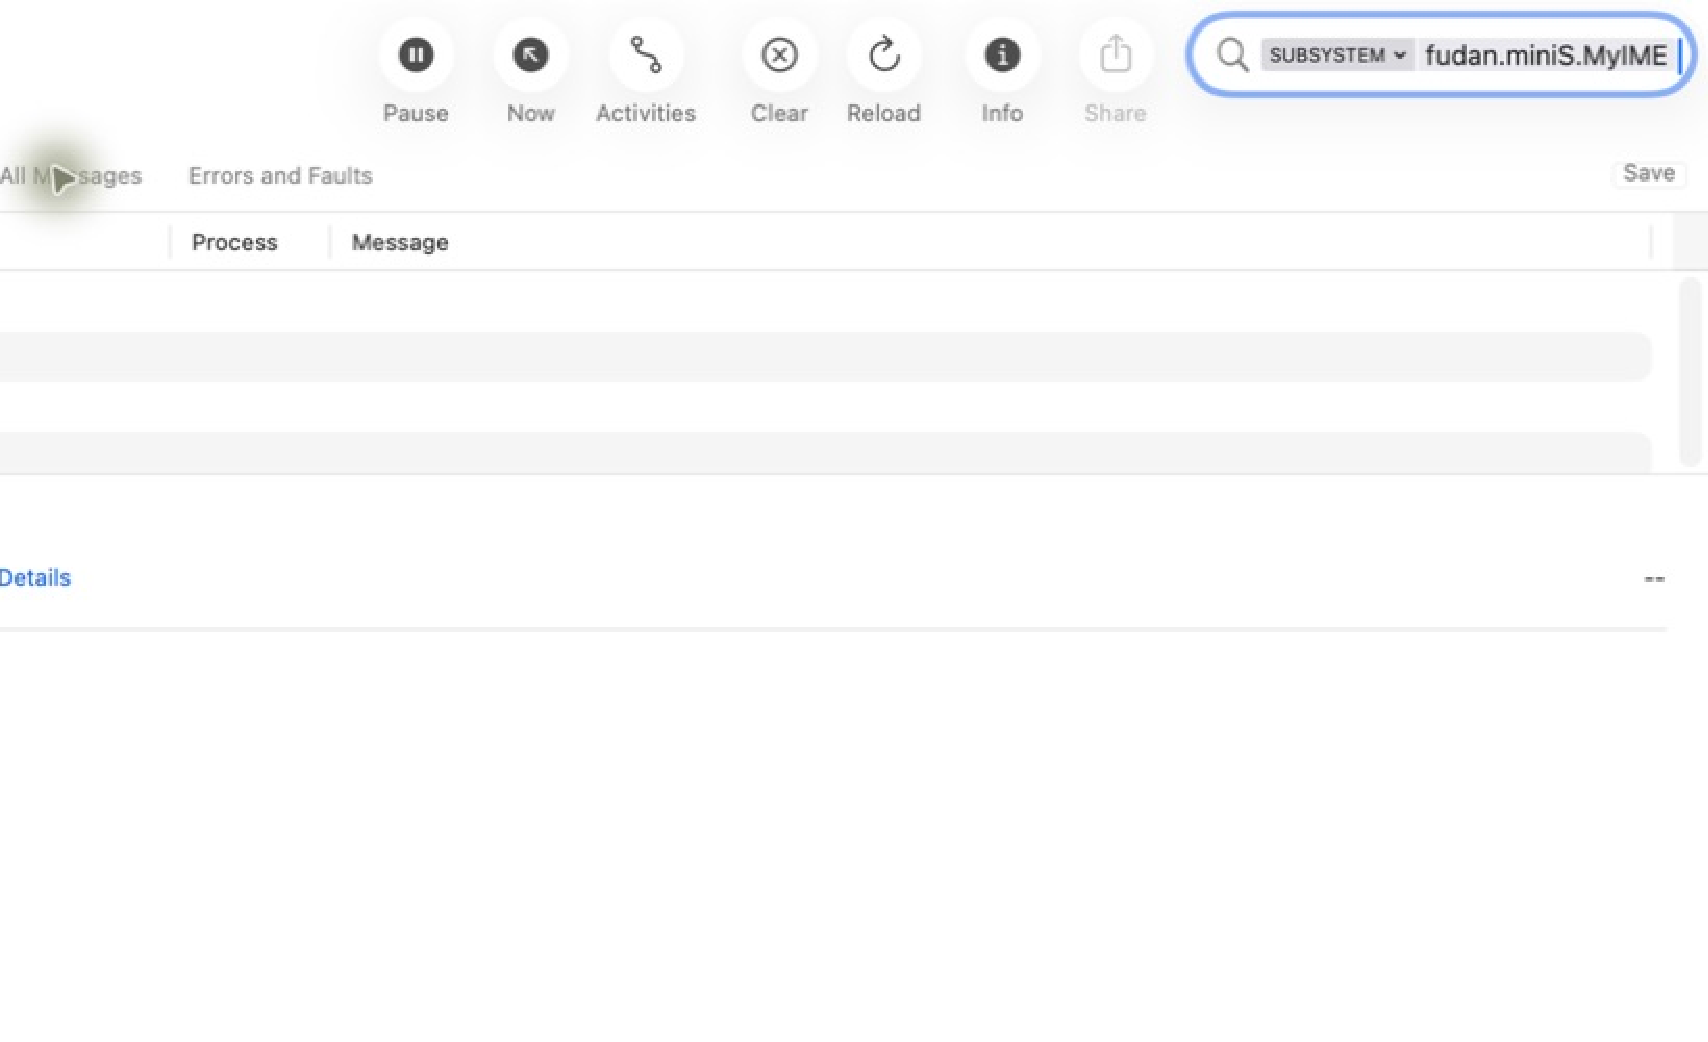
\includegraphics[width=\linewidth]{assets/console-filter.pdf}
  \caption{Console.app 以 subsystem 过滤 MyIME 日志；截图已裁去机器名称}
\end{figure}

一轮复现应形成以下最小证据链：\code{bootstrap server ready} → \code{controller keyDown} → \code{engine candidates=N} → \code{client marked/insert}。若第一项都没有，查进程和 IMKServer；有第一项而没有第二项，查当前输入源与事件入口；有候选却没有客户端调用，查控制器状态和事件返回值。导出日志前必须再次搜索正文样例和用户名，确认脱敏。

\section{诊断问题树}

面对“没有 MyIME”时依次问：

\begin{enumerate}
  \item 安装目录是否存在应用，版本和签名是什么？
  \item TIS 是否枚举到目标输入源 ID？
  \item 当前输入源 ID 是否为 MyIME？
  \item 进程路径是否来自安装目录？IMKServer 是否建立？
  \item 按键进入哪个回调？控制器返回了什么？
  \item 引擎输出候选是否为空？资源库是否完整？
  \item 客户端收到 marked text/insert text 了吗？
\end{enumerate}

面对“候选不对”则从第 5 步开始：归一化 raw、切分路径、SQL 召回、分数分解、后处理和 UI 映射。

\section{隐私友好的日志}

Release 日志可记录：输入长度、路径数量、候选数量、耗时、错误码、应用 Bundle ID 和状态转移；不应默认记录用户完整 raw、候选文本、剪贴板或已提交句子。必要的用户诊断应采用明确同意、短时开启和本地导出。

\begin{concept}[关联 ID]
为一次输入会话生成短关联 ID，使 bootstrap、controller、engine 和 store 日志能够串联，而无需写出正文。例如：\code{session=7F2A, rawLength=8, paths=3, candidates=25, p95Bucket=20ms}。
\end{concept}

\section{死锁与卡顿调试 SOP}

\textbf{先分症状。}崩溃、数据竞争、逻辑死锁和主线程长任务是四类问题，不能只靠同一个工具。复现前固定输入、客户端、系统版本和构建号，并保存正常基线。

\begin{enumerate}
  \item 在 Xcode 的 Scheme→Run→Diagnostics 打开 Thread Sanitizer（TSan），用 Debug 构建重放并发选择、异步学习和数据库故障。TSan 擅长发现未同步的共享内存访问，但不能证明所有逻辑死锁都不存在。命令行可用 \code{xcodebuild ... -enableThreadSanitizer YES test}。TSan 会显著拖慢程序，只用于诊断构建。\footnote{Apple：\url{https://developer.apple.com/documentation/xcode/diagnosing-memory-thread-and-crash-issues-early}}
  \item 若界面已经卡住，在 Xcode 点击 Pause，展开所有线程。记录主线程调用栈、持锁线程和等待栈；若线程 A 等待由 A 自己持有的非递归 \code{NSLock}，就是重入；若 A 等 B、B 又等 A，则画出等待环。不要在锁内调用客户端、SQLite、日志插值闭包或未知回调。
  \item 打开 Main Thread Checker，捕获从后台线程触碰 \code{NSPanel}/SwiftUI 的路径。它检查 UI 线程契约，和 TSan 的数据竞争检查互补。
  \item 对“能动但很慢”选择 Product→Profile→Time Profiler。只录制 10--20 秒：先空闲 3 秒，再输入固定长句，最后空闲 3 秒。按进程过滤 MyIME，展开 Main Thread；重点查 \code{sqlite3_step}、锁等待、候选排序和 SwiftUI 布局是否占据热栈。Apple 也建议用 Time Profiler 分析无响应与挂起。\footnote{Apple：\url{https://developer.apple.com/documentation/xcode/improving-your-app-s-performance/}}
  \item 修改后用相同机器、输入和采样窗口复测，比较 P50/P95 与主线程最重栈，而不是只报告“感觉顺了”。再关闭 Sanitizer 运行一次 Release 配置，排除诊断开销造成的假象。
\end{enumerate}

\begin{warningbox}[NSLock 重入的典型陷阱]
线程在持有 \code{NSLock} 时调用一个看似只读的辅助函数，而该函数为了读取同一状态再次加锁，会永久等待。把锁保护的不变量写在字段旁；锁内只复制/更新小状态，解锁后再调用数据库、客户端和 UI。
\end{warningbox}

\section{诊断工具}

仓库提供输入源检查、注册和本地安装工具。工具输出应被视作辅助证据，而不是绕过正常系统路径的永久依赖。正式版不能靠一个登录守护进程不断强制恢复，因为这会隐藏生命周期设计缺陷。

\lstinputlisting[language=Swift,firstline=1,lastline=120,caption={输入源检查工具示例}]{../../tools/inspect_input_source.swift}

\begin{lab}[故障注入]
分别制造词库缺失、用户库只读、错误输入源 ID 和候选坐标失败。为每个故障写出预期日志和用户可见降级，验证不会让所有按键失效。
\end{lab}

\exercises
\begin{enumerate}
  \item 日志中记录 raw 的 SHA-256 是否绝对安全？为什么？
  \item 设计一个一键生成的本地诊断报告目录结构。
  \item “进程存在但没有回调日志”下一步应收集什么证据？
\end{enumerate}

\begin{summarybox}
好的诊断系统把模糊故障变成逐层证据链，并把可观察性与隐私同时纳入设计，而不是发生问题后临时加 print。
\end{summarybox}


\chapter{隐私、安全与词库许可证}

\begin{goals}
理解输入法的高敏感权限；能够建立完全离线的威胁模型；识别安全输入、日志、更新包、用户数据库和第三方词库中的风险。
\end{goals}

输入法位于所有文本之前，理论上可能接触私人通信、搜索、地址和代码。即使产品承诺离线，也必须用架构和可验证事实支持承诺：没有网络依赖、没有隐蔽上传路径、日志不保存正文、更新包经过签名、用户库权限正确。

\section{威胁模型}

至少考虑以下资产与攻击面：

\begin{itemize}
  \item 用户原始按键、候选选择和提交文本；
  \item 用户词库与上下文数据库；
  \item 应用内置系统词库和替换词库入口；
  \item 安装器的文件替换权限；
  \item 发布服务器、GitHub Release 和 DMG 供应链；
  \item 调试日志、崩溃报告与课堂演示录像。
\end{itemize}

完全离线可以显著缩小攻击面，但不能自动解决本地恶意软件、宽松文件权限、未签名更新和敏感日志。用户数据库应存放在当前用户目录，避免其他普通账户读取；导出时应明确提示内容敏感。

\section{安全输入}

密码字段可能启用 Secure Event Input 或拒绝第三方组合。输入法应尊重该边界，不尝试绕过；无法输入时回退系统安全键盘是正确行为。教学演示禁止在真实密码框记录事件日志。

\section{开源与词库许可}

输入法代码开源不等于所有聚合词库都可以任意再分发。MyIME 的流水线记录来源锁、许可证和派生步骤，应用内附第三方声明。

\lstinputlisting[language=bash,firstline=1,lastline=95,caption={词库来源与许可清单的一部分}]{../../tools/LICENSES.md}

课堂项目应为每个来源记录：名称、URL、版本/提交、许可证、是否修改、输出中保留什么以及再分发义务。无法确认许可的词表不得进入正式发布包。

\begin{lab}[离线审计]
在干净用户账户中运行输入法，使用系统网络观察工具检查进程连接；搜索源码中的 URLSession、Network 和 socket 调用；检查 Release 包中第三方声明与词库来源是否一致。
\end{lab}

\exercises
\begin{enumerate}
  \item “不上传击键”与“完全没有网络请求”有什么区别？
  \item 用户主动导出词库是否改变应用的隐私责任？
  \item 为可下载的离线词库更新包设计签名验证流程。
\end{enumerate}

\begin{summarybox}
输入法的隐私承诺必须由网络边界、日志策略、文件权限、供应链和许可证记录共同支撑。离线是强优势，但不是安全证明的终点。
\end{summarybox}


\chapter{测试体系：从内存词库到跨机器验收}

\begin{goals}
建立单元、集成、性能和人工验收四层测试；掌握 golden、性质测试、故障注入和确定性；把历史故障转化为回归用例。
\end{goals}

输入法核心适合大量自动化测试，系统集成则需要少量高价值人工测试。测试金字塔底层包含切分、排序、用户学习和数据库；中层构建应用并检查资源、签名和架构；顶层在真实客户端敲固定序列。

\figmp{11}{自动化与人工测试的合理比例}

\section{行为测试}

MyIME 的内存词库让测试只包含与行为有关的词。Golden 测试锁定 \code{nihao}→“你好”等核心首选；上下文测试故意让“田七”静态权重更高，再由“今天”上下文把“天气”提升回来。

\lstinputlisting[language=Swift,firstline=103,lastline=174,caption={整句、上下文与续写测试}]{../../MyIME/IMEKit/Tests/IMEKitTests/IMEKitTests.swift}

\section{性质与故障测试}

固定样例覆盖已知场景，性质测试覆盖不变量。例如对随机 ASCII 字符串：引擎不崩溃、耗时不超过预算、消费长度不越界、同输入与同状态结果确定。对损坏数据库：引擎降级，不阻塞基本输入。

\section{性能测试}

性能断言应在可控环境执行，避免把 CI 机器偶发负载当作算法回归。更稳健的做法是记录分布并设置宽松硬门槛，同时在版本间比较相对变化。冷启动、热查询和长句需要分别统计。

\section{跨机器门禁}

发布前必须在不含开发证书、不含旧输入法副本的第二台 Mac 上，从 GitHub Release 下载 DMG，完成安装、注册和 Notes 输入。开发机成功不能替代跨机器验收，因为钥匙串、LaunchServices 缓存和旧构建都可能掩盖问题。

\begin{lab}[把 bug 变成测试]
选择一次历史故障，例如进程被结束后不能恢复、换机后输入源不出现或 Notes 无法组合。先写最小复现，再决定哪一部分能自动化，哪一部分保留为发布清单。
\end{lab}

\exercises
\begin{enumerate}
  \item Golden 测试过多会带来什么维护问题？
  \item 如何测试候选排序确定性？
  \item 为什么跨机器验收属于发布门禁，而不是“有空再测”？
\end{enumerate}

\begin{summarybox}
测试体系要让算法快速回归、系统问题可复现、发布风险可阻断。每个真实故障都应留下自动化测试或明确人工门禁。
\end{summarybox}


\chapter{签名、公证、Universal 2 与 DMG 发布}

\begin{goals}
理解开发签名、Developer ID、公证和装订的区别；能够解释 Universal 2；掌握可重复发布流水线与校验和。
\end{goals}

能在开发机运行的应用不等于可以跨机器分发。公开 DMG 应使用 Developer ID Application 证书签名，提交 Apple 公证，成功后把票据装订到应用或镜像，并验证 Gatekeeper 接受。

\figmp{12}{从测试到公开 DMG 的发布门禁}

\section{签名身份}

Apple Development 证书用于开发调试；Developer ID Application 用于 App Store 外分发。Ad-hoc 签名只证明代码页一致，不建立公开开发者信任。发布脚本必须主动拒绝把 development 或 ad-hoc 构建标为正式版。

\section{Universal 2}

Universal 2 应用同时包含 arm64 和 x86\_64 代码。仅把文件名写成 universal 不够，需要用 \code{lipo -info} 或 \code{file} 检查主可执行文件和嵌入的本地库。SQLite 等系统动态库通常由系统提供，但自带二进制依赖也必须双架构。

\section{发布脚本}

MyIME 的脚本按顺序运行引擎测试、词库验证、构建、架构检查、签名、DMG、公证、装订和 SHA-256。顺序本身就是安全性质：任何前置门禁失败都不应继续发布。

\lstinputlisting[language=bash,firstline=1,lastline=220,caption={正式发布脚本的环境检查与主要门禁}]{../../tools/build-release.sh}

\section{凭据管理}

公证凭据应存入钥匙串 profile，而不是写进脚本或提交到仓库。应用专用密码一旦出现在截图或聊天记录中，应立即撤销并重新生成。课堂作业不要求学生共享教师证书；每组可生成 ad-hoc 演示包，正式公开发布由项目维护者在受控机器执行。

\begin{warningbox}[公证成功不代表功能成功]
公证只证明 Apple 的安全检查接受该二进制，不证明输入源能注册、候选准确或 Notes 可输入。最终门禁仍包含目标机功能验收。
\end{warningbox}

\begin{lab}[验收一个 Release]
对 DMG 依次运行 \code{shasum -a 256}、\code{spctl --assess}、\code{codesign --verify --deep --strict}、\code{xcrun stapler validate}。挂载后检查应用版本、架构与签名团队，再在干净 Mac 安装。
\end{lab}

\exercises
\begin{enumerate}
  \item 签名、公证和装订分别解决什么问题？
  \item 为什么发布凭据不能通过环境变量明文保存在 CI 日志？
  \item 设计一份可由第三方复核的 Release 清单。
\end{enumerate}

\begin{summarybox}
正式发布是一条不可跳步的证据链。测试、双架构、Developer ID、Apple 公证、票据装订、校验和和跨机器输入共同定义“可下载版本”。
\end{summarybox}


\chapter{维护真实输入法：技术债与演进边界}

\begin{goals}
能够评审控制器和安装器中的复杂度；区分教学最小实现与生产兼容代码；设计版本迁移、文档同步和未来功能边界。
\end{goals}

MyIME 作为教学案例的价值在于它既有清晰核心，也暴露真实复杂度。\sourcefile{Engine.swift}、\sourcefile{MyIMEInputController.swift} 和 \sourcefile{SelfInstaller.swift} 已经包含大量策略。继续增加双拼、云更新或移动平台前，应先检查模块边界，而不是把新分支堆进控制器。

\section{复杂度地图}

\begin{center}
\begin{tabularx}{\linewidth}{p{3cm}X X}
\toprule
模块 & 当前职责 & 演进建议 \\
\midrule
InputController & 事件、组合、候选导航、客户端适配、英文辅助 & 抽出 InputAction 与 CompositionState，降低分支耦合 \\
Engine & 切分协调、词查询、评分、词格、上下文、学习 & 保持纯逻辑；为评分解释和策略注入留接口 \\
SQLiteStore & 系统查询、统计模型、用户库 & 分离只读 schema 与用户迁移版本 \\
SelfInstaller & 复制、注册、旧版迁移、重启 & 用明确安装阶段和错误类型替代隐式布尔状态 \\
候选窗口 & SwiftUI 渲染与 AppKit 窗口定位 & 增加可访问性与多屏快照测试 \\
\bottomrule
\end{tabularx}
\end{center}

\section{规格、实现与测试同步}

仓库中的 \sourcefile{SPEC.md} 描述目标，\sourcefile{FOOLPROOFING.md} 描述门禁，README 描述用户能力，代码是实际行为。它们可能随版本产生漂移。维护者应给每项功能标记 implemented、planned 或 removed，并把用户可见变化写入版本说明。

\section{功能边界}

双拼会改变切分与设置，但不必改变 IMK 生命周期；云词库会改变隐私承诺和更新安全；语音输入引入音频权限与服务端/本地模型；移动端输入法则是不同平台架构。评审新功能时先问它改变哪一层契约，再决定是否仍属于同一个产品。

\begin{concept}[教学版与完整版共存]
最好的教材仓库不是把生产代码削成玩具，而是保留两个视图：章节化的教学版展示关键原理，完整版展示边界条件和发布现实。学生先能解释，再能维护。
\end{concept}

\section{把无障碍作为回归契约}

候选列表的“能看见、能点击”不等于可访问。每个候选行应是独立无障碍元素，标签读出序号与候选词，当前高亮项增加 \code{.isSelected} trait；辅助说明放在 hint，不要把词频、调试分数等噪声塞进主标签。SwiftUI 示例见第 7 章。

当方向键改变高亮时，可按需发送 \code{NSAccessibility.announcementRequestedNotification}，\code{userInfo} 中提供 announcement 与 priority。\footnote{Apple：\url{https://developer.apple.com/documentation/appkit/nsaccessibilityannouncementrequestednotification}}公告必须节流：按键长按时只读最终稳定项，避免 VoiceOver 被消息队列淹没。非激活 \code{NSPanel} 不应抢走宿主编辑器焦点；关闭候选窗后，VoiceOver 焦点仍应留在原文本控件。

每次改候选 UI 至少回归：VoiceOver 开/关、键盘全访问、提高对比度、减少透明度、浅色/深色、多屏与放大显示。自动化测试可验证 label、selected trait 和稳定候选索引，人工测试负责朗读顺序、焦点保持与语速下的可理解性。

\begin{lab}[架构评审]
选择一个计划功能（双拼、词库导入、诊断面板或用户词导出），写一页变更契约：目标、涉及模块、不改变的行为、数据迁移、测试和发布风险。禁止先写代码。
\end{lab}

\exercises
\begin{enumerate}
  \item 哪些控制器状态可以抽成纯 Swift 状态机？
  \item 加入双拼时，Candidate 的 pinyinPath 是否仍足够？
  \item 如何避免教材行号随源码变化失效？提出一种自动检查办法。
\end{enumerate}

\begin{summarybox}
真实输入法的维护重点不是持续增加功能，而是守住系统、算法、存储和发布契约。教学最小版解释原理，完整版本训练工程判断。
\end{summarybox}


\part{课程实验与综合项目}
\chapter{实验一至四：从 Echo 到候选窗口}

本章给出初级篇的可提交实验。每个实验都要求“源码、测试、观察记录”三件套。只提交能运行的 App 不足以证明理解；只提交报告也不足以证明实现。

\section{从哪个分支开始}

仓库提供 \code{lab1-starter} 至 \code{lab12-starter} 十二个起始分支；分支名表示“开始该实验前的状态”，不表示答案。学生只克隆教师指定的 starter，并从自己的作业分支提交：

\begin{lstlisting}[language=bash,numbers=none]
git fetch origin --prune
git switch --create homework/lab1 origin/lab1-starter
swift test --package-path TeachingStarter
\end{lstlisting}

\begin{center}
\small
\begin{tabular}{p{2.8cm}p{4.2cm}p{5.2cm}}
\toprule
Starter & 已提供的边界 & 学生完成的核心 \\
\midrule
\code{lab1-starter} & IMK 配置清单与 Echo 接口 & 最小服务器、事件回送 \\
\code{lab2-starter} & 纯状态机类型与表测框架 & 组合、退格、提交、取消 \\
\code{lab3-starter} & 小词库协议与 TSV fixture & 候选召回、稳定排序 \\
\code{lab4-starter} & 候选 ViewModel 与坐标 fixture & 不抢焦点窗口、多屏定位 \\
\code{lab5-starter} & 音节表和图搜索接口 & 切分图、撇号、简拼与容错 \\
\code{lab6-starter} & \code{ScoreBreakdown} 数据型 & 分数解释与消融 \\
\code{lab7-starter} & 小词格 fixture & Beam Search 与完整枚举校验 \\
\code{lab8-starter} & 临时用户库 schema & 异步学习、清空与故障降级 \\
\code{lab9-starter} & 客户端测试矩阵模板 & 跨客户端、VoiceOver 回归 \\
\code{lab10-starter} & 诊断报告字段协议 & 脱敏收集与证据链 \\
\code{lab11-starter} & 许可证/SBOM 清单模板 & 离线与供应链审计 \\
\code{lab12-starter} & Release 验收脚本骨架 & 第二台 Mac 安装和恢复 \\
\bottomrule
\end{tabular}
\end{center}

完整 MyIME 1.0.10 用于课后对照，不是实验起点。公开仓库中的分支只能避免“误入完整实现”，不能阻止刻意查看 \code{main}；正式评分课程应把对应 starter 导入独立的 GitHub Classroom 私有模板仓库，只向学生开放模板。教师的 solution 分支不要推送到学生可读仓库。

\section{实验一：Echo IME}

\textbf{目标：}建立最小 IMKServer 和控制器，在 Notes 中原样回送字母。

\textbf{约束：}不得引入数据库、候选窗口或自动安装器；核心代码不超过 150 行；必须记录真正进入的回调。

\textbf{步骤：}

\begin{enumerate}
  \item 新建 macOS App target，配置输入源 plist；
  \item 创建 IMKServer，并在入口日志记录 bundle path、bundle ID 和 connection name；
  \item 控制器只处理可打印 ASCII，其他事件放行；
  \item 安装到用户输入法目录，重新登录或注册；
  \item 在 Notes 输入 \code{hello 123}，验证无重复和丢字。
\end{enumerate}

\textbf{验收问题：}返回 true/false 的区别是什么？进程存在为何不足以证明事件进入控制器？

\section{实验二：组合状态}

\textbf{目标：}实现 raw buffer、marked text、退格、Esc 和 Return。

建议先在纯 Swift 中实现：

\begin{lstlisting}[language=Swift,caption={教学状态机接口}]
enum InputAction: Equatable {
    case append(Character), deleteBackward, commit, cancel
}

struct CompositionState: Equatable {
    var raw = ""
    mutating func reduce(_ action: InputAction) -> Effect { /* ... */ }
}

enum Effect: Equatable {
    case updateMarked(String), insert(String), clearMarked, none
}
\end{lstlisting}

用表驱动测试覆盖空闲态与组合态。随后写一个薄适配器，把 Effect 映射到 \code{setMarkedText} 或 \code{insertText}。

\section{实验三：小词库候选}

\textbf{目标：}使用不超过 100 条 TSV 词库完成全拼候选和数字选词。

\textbf{必测输入：}\code{nihao}、\code{beijing}、一个同音词、一个不存在的拼音、一个未完成前缀。候选排序必须有稳定 tie-breaker。报告中展示每个候选的权重和最终排序原因。

\section{实验四：候选窗口}

\textbf{目标：}实现不抢焦点的候选窗、方向键高亮、数字选择、翻页和屏幕边缘定位。

\textbf{截图要求：}屏幕中央、左下角、右下角、多显示器各一张。截图必须同时包含插入点和候选窗，证明没有越界。

\section{评分量表}

\begin{longtable}{p{4cm}p{1.5cm}p{6cm}}
\toprule
项目 & 分值 & 判定 \\
\midrule
输入源可注册、可选择 & 15 & 使用稳定 ID，无重复条目 \\
事件所有权正确 & 15 & 无重复、无吞键，修饰键放行 \\
组合状态正确 & 20 & 退格、取消、提交和失活一致 \\
候选与部分输入 & 15 & 小词库结果稳定且可解释 \\
窗口交互 & 15 & 不抢焦点、可导航、不越界 \\
自动化测试 & 10 & 状态机与词库至少 12 个测试 \\
实验报告 & 10 & 有失败证据、原因和修复验证 \\
\bottomrule
\end{longtable}


\chapter{实验五至八：切分、排序、整句与学习}

\section{实验五：切分图}

输入一组拼音，输出 DOT 或文本形式的切分图。至少覆盖全拼、多路径、撇号、简拼、混拼、模糊音和一次错拼。要求验证：完整消费优先、结果确定、非法字符不崩溃。

\textbf{扩展任务：}实现递归搜索与动态规划两种方法，对 1 万条随机输入比较输出与耗时。若结果不同，必须给出反例并解释。

\section{实验六：评分解释器}

为每个候选输出：

\begin{lstlisting}[numbers=none]
word=天气
frequency=-3.42
user=+0.00
context=+2.18
fuzzy=-0.00
partial=-0.00
incomplete=-0.00
total=-1.24
\end{lstlisting}

选择至少十组同音/近音候选，通过消融实验说明每项存在的必要性。调参结论必须来自开发集，不得根据封存测试集逐条修改。

\section{实验七：词格整句}

实现宽度可配置的 Beam Search。测试 \code{woshizhongguoren}、\code{jintiantianqihenhao} 和一条至少 10 音节句子。记录 Beam 宽度为 2、4、8、12、24 时的 top-1、top-5、P50 和 P95。

\textbf{正确性检查：}使用一个很小的词格完整枚举所有路径，与 Beam 宽度足够大时的结果比较。这是用第二种方法验证搜索实现，而不是只相信几个 golden 用例。

\section{实验八：用户学习}

实现用户 unigram、bigram 和最近组词之一。必须支持重启持久化和清空。为数据库故障注入只读、损坏文件和并发选择，证明基本输入仍可用。

\section{实验报告模板}

每个实验按以下结构提交：

\begin{enumerate}
  \item 问题定义与不变量；
  \item 两种实现或验证方法；
  \item 数据集与环境；
  \item 结果表和至少一幅图；
  \item 失败案例与原因；
  \item 对完整 MyIME 源码的对应关系；
  \item 残余风险与下一步。
\end{enumerate}


\chapter{实验九至十二：兼容、诊断、安全与发布}

\section{实验九：跨客户端兼容矩阵}

选择 Notes、TextEdit、Safari、Chrome、一个 Electron 应用和一个国产办公/通信应用。固定测试 12 条输入序列，包括中英文切换、长句、退格、候选导航、应用切换和进程恢复。

\begin{center}
\begin{tabular}{lcccccc}
\toprule
用例 & Notes & TextEdit & Safari & Chrome & Electron & 其他 \\
\midrule
首选上屏 & & & & & & \\
退格刷新 & & & & & & \\
候选定位 & & & & & & \\
应用切换 & & & & & & \\
进程恢复 & & & & & & \\
\bottomrule
\end{tabular}
\end{center}

每个失败必须附最小输入序列和事件路径日志。禁止用“兼容性不好”作为结论。

候选窗口还须在 VoiceOver 下验证：方向键改变高亮时朗读序号与候选，selected 状态可识别，候选窗出现/消失不夺走宿主编辑器焦点。把该结果作为矩阵的一行，而不是只写进文字备注。

\section{实验十：诊断包}

实现一个不包含正文的本地诊断命令，输出：应用版本与路径、签名摘要、当前输入源 ID、TIS 枚举结果、系统版本、芯片架构、词库完整性、用户库 schema 版本和最近 200 行脱敏日志。

在报告中给出威胁分析：哪些字段仍可能间接识别用户？诊断包如何过期和删除？

\section{实验十一：离线与供应链审计}

检查源码依赖和运行时网络连接；确认 Release 包中的第三方许可；验证替换词库入口不能加载损坏或未经验证的文件。对下载 DMG 计算 SHA-256，并与发布页校验和比较。

\section{实验十二：第二台 Mac 发布验收}

目标机器必须满足：没有开发证书、没有源码、没有旧 MyIME 副本。只能从公开 Release 下载 DMG。验收步骤如下：

\begin{enumerate}
  \item 验证 SHA-256、Developer ID 与公证票据；
  \item 打开 DMG 并安装，不使用 Xcode 或本地脚本；
  \item 在系统设置确认 MyIME 位于简体中文分类；
  \item 在 Notes 输入规定句子并录屏；
  \item 结束输入法进程，通过 ABC→MyIME 恢复；
  \item 重启机器后再次验证；
  \item 卸载并确认用户选择的数据保留/删除策略符合说明。
\end{enumerate}

\begin{warningbox}[凭据纪律]
学生不得在报告、截图、录屏或 Git 历史中包含 Apple ID 密码、应用专用密码、证书私钥或钥匙串导出文件。发生泄露应立即撤销，而不是仅删除截图。
\end{warningbox}


\chapter{综合项目：实现一款可解释的离线输入法}

\begin{goals}
把课程知识转化为独立设计；形成可运行软件、可复现评测和可审查发布物；能够在答辩中用证据说明每个关键决策。
\end{goals}

综合项目可以在 MyIME 上实现一个明确增量，也可以从教学版继续发展。推荐题目包括：双拼支持、用户词导入导出、评分解释面板、专业领域离线词库、可访问候选窗口、离线词库签名更新、组合状态机重构或跨客户端自动化测试工具。

\section{项目契约}

立项书不超过两页，必须包含：用户问题、范围、明确不做的功能、受影响模块、数据结构变化、隐私变化、测试指标和演示路径。若题目引入网络能力，必须单独通过隐私与安全评审。

\section{最终交付物}

\begin{enumerate}
  \item 可构建源码与清晰提交历史；
  \item 设计说明，包含架构图、状态机或算法图；
  \item 自动化测试与完整命令输出；
  \item 至少 200 条封存集评测和延迟分布；
  \item 跨机器兼容矩阵；
  \item 签名/公证发布物或明确标记的开发演示包；
  \item 三分钟演示视频与十分钟技术答辩。
\end{enumerate}

\section{100 分三级评分量表}

“卓越”通常获得该项 85--100\% 分值，“合格”获得 60--84\%，“不合格”获得 0--59\%。严重安全事故、无法构建或伪造数据可触发课程规则中的额外封顶；助教必须在评语中引用具体提交证据，不能只写主观印象。

{\small
\setlength{\tabcolsep}{3pt}
\begin{longtable}{p{2.1cm}p{.8cm}p{3.25cm}p{3.25cm}p{3.25cm}}
\toprule
维度 & 分 & 卓越 & 合格 & 不合格 \\
\midrule
\endfirsthead
\toprule
维度 & 分 & 卓越 & 合格 & 不合格 \\
\midrule
\endhead
问题与范围 & 10 & 用户问题、非目标、成功指标和变更契约均可验证；范围变化有记录 & 目标基本明确，能演示主要路径；少量非目标或指标模糊 & 只有功能口号；范围持续漂移，无法判定完成 \\
架构 & 15 & 系统/算法/存储/UI 边界明确；主线程、锁和失败降级有图与不变量 & 能说明主要模块，依赖方向大体合理；存在局部耦合但可维护 & 控制器包揽全部逻辑；共享状态无所有权，修改一处破坏多处 \\
核心正确性 & 20 & 正常、边界、失败路径齐全；关键算法由完整枚举、模型或第二实现交叉验证 & 主流程和常见边界正确；测试覆盖主要不变量，但验证方法单一 & 吞键、重复上屏、崩溃或错误提交可稳定复现；只靠演示样例 \\
准确率与性能 & 15 & 训练/开发/封存集隔离；报告 top-k、P50/P95/P99、样本量及误差分析；优化有前后对照 & 有固定数据集与 P95；结果可复现，但分层/误差分析不完整 & 用挑选样例或“感觉更快”代替指标；测试集被用于逐例调参 \\
系统兼容 & 10 & 多客户端、多屏、生命周期、VoiceOver 和第二台 Mac 均有最小复现证据 & Notes 加至少两类客户端通过；恢复和坐标边界有基本验证 & 仅开发机单一文本框可用；依赖守护进程或手工脚本维持 \\
隐私与安全 & 10 & 数据流、日志脱敏、文件权限、许可、签名/公证和凭据撤销策略完整 & 无网络或网络用途清楚；无正文日志和已知明文凭据；许可基本齐全 & 上传/记录正文未告知；提交密码、私钥；来源或许可无法说明 \\
测试工程 & 10 & 纯逻辑、存储、系统适配分层；历史故障有回归；失败输出可定位且无顺序依赖 & 自动化覆盖核心模块并能一键运行；少量系统步骤仍需人工 & 测试不能运行、依赖个人机器状态，或只有截图无断言 \\
表达与答辩 & 10 & 能从按键到上屏逐层解释，并现场说明分数、剪枝、锁、SQL 和发布证据 & 能解释主要设计与已知限制；在提示下可定位源码和测试 & 无法区分 marked/commit、事件所有权或发布签名；报告与实现矛盾 \\
\bottomrule
\end{longtable}
}

\section{答辩必问十题}

\begin{enumerate}
  \item 当前按键由哪个入口收到，为什么？
  \item 返回 true/false 会怎样？
  \item raw、preedit、marked text 和 commit 分别存在哪里？
  \item 展示一个候选的完整分数分解。
  \item 展示一个切分歧义和一个词格剪枝。
  \item 用户词库损坏时怎样降级？
  \item 哪些日志可能泄露隐私？
  \item 为什么开发机成功不能证明 Release 成功？
  \item 你的测试集如何避免泄漏？
  \item 如果再给两周，你会优先消除哪个风险？
\end{enumerate}

\begin{summarybox}
综合项目的目标不是复制 MyIME 功能数量，而是证明学生能够用系统模型、算法、测试和发布证据完成一个可信的输入法增量。
\end{summarybox}


\appendix
\chapter{Swift 与并发速查}

本附录只收录理解 MyIME 必需的 Swift 概念。

\section{值类型与引用类型}

\code{struct} 复制值，适合 Candidate、EngineOutput 和偏好快照；\code{class} 具有对象身份，适合控制器、数据库连接和窗口控制器。包含数组的结构体仍享受写时复制，但跨线程安全要看元素与访问方式。

\section{协议与 existential}

\code{any CandidateLookup} 表示运行时持有任意满足协议的对象；泛型 \code{Engine<Store: CandidateLookup>} 则在编译期特化。前者便于替换与保存，后者可能有性能优势。输入法查询开销主要在数据库与搜索，当前 existential 通常不是瓶颈。

\section{可选值与 guard}

系统 API 大量返回可选值。控制器入口宜用 guard 验证 client、字符和范围，把失败路径尽早放行或降级。不要为了减少代码而强制解包客户端对象。

\section{Sendable、锁与队列}

\code{Sendable} 表示值可以安全跨并发域传递；\code{@unchecked Sendable} 表示作者自行保证。常见保护方法包括：

\begin{itemize}
  \item 不可变值快照；
  \item \code{NSLock.withLock} 保护小型同步状态；
  \item 串行 DispatchQueue 保护 SQLite 写入；
  \item Actor 隔离异步状态；
  \item \code{@MainActor} 限制 UI 和 App 生命周期。
\end{itemize}

\begin{warningbox}
不要在持有状态锁时执行 SQL、调用客户端或刷新 UI。锁的临界区只读写必要字段，避免重入和主线程卡顿。
\end{warningbox}

\section{输入法线程模型：先画所有权，再写并发代码}

输入法没有“所有工作都在后台越快越好”这一选项。IMK 事件回调、NSPanel 和 SwiftUI 更新属于 UI/会话层，MyIME 用 \code{@MainActor} 把它们限制在主执行器；用户数据库写入可以串行异步执行；引擎计算保持同步、短小，并以不可变 \code{EngineOutput} 快照返回 UI。

\figmp{14}{MyIME 的线程模型：主执行器处理会话与 UI，UserStore 队列串行持久化}

\begin{longtable}{p{3.1cm}p{3.4cm}p{4.6cm}}
\toprule
对象/操作 & 推荐执行域 & 原因与约束 \\
\midrule
IMK 回调、客户端调用 & MainActor & 输入会话有严格顺序，客户端对象不可跨线程长期持有 \\
\code{CandidateWindow}/\newline\code{NSPanel} & MainActor & AppKit UI 必须在主线程更新 \\
Engine.update & 调用线程，受时间预算限制 & 返回值快照；不得在其中等待异步写入 \\
提交历史 & NSLock 短临界区 & 只复制/更新少量值，禁止锁内 SQL 和 UI \\
UserStore.learn & 私有串行队列 & 保证 SQLite 写入顺序，不阻塞按键路径 \\
system.sqlite 查询 & 连接所有者线程/受控同步 & 只读；同一 statement 不得无保护并发复用 \\
\bottomrule
\end{longtable}

\subsection{@MainActor、Sendable 与 @unchecked Sendable 分别保证什么}

\code{@MainActor} 是隔离规则：编译器要求相关状态和方法在主执行器访问。\code{Sendable} 是跨并发边界的值安全承诺；像 Candidate 这样的不可变结构体适合自动满足。\code{@unchecked Sendable} 则表示“编译器不再证明，由作者负责”，必须在代码评审中附带同步策略。它绝不能成为消除警告的通用修饰符。

\subsection{NSLock 的两条铁律}

第一，锁保护的是一个写明的不变量，而不是“这一整个函数”；第二，不调用未知代码。客户端、闭包、日志格式化和 SQLite 都可能重入或阻塞。正确形式是锁内复制状态、立即解锁，再执行外部操作：

\begin{lstlisting}[language=Swift,caption={缩短锁临界区}]
let history = stateLock.withLock { committedHistory }
// 锁已经释放；下面可以查词、评分和刷新 UI。
let anchors = contextAnchors(last: history.last,
                             beforeLast: history.beforeLast)
\end{lstlisting}

\begin{lab}[画线程所有权图]
从一次候选选择开始，标出回调线程、Engine、NSLock、UserStore 队列和 SQLite。对每条跨域箭头写出传递的数据类型；若传的是 client、NSWindow 或可变数组，说明为何危险并改成值快照。
\end{lab}

\section{String 索引}

Swift String 按扩展字素簇索引，不支持任意整数下标。raw 被归一化为 ASCII 时可以安全按字符数量推导消费长度；汉字候选的 \code{count} 是字符数量，不等于 UTF-8 字节数。数据库和 C API 交界处必须明确编码单位。


\chapter{InputMethodKit 与 TIS 速查}

\section{核心类型}

\begin{longtable}{p{4cm}p{7.2cm}}
\toprule
类型/方法 & 教学意义 \\
\midrule
\code{IMKServer} & 注册输入法服务连接，由系统发现控制器 \\
\code{IMKInputController} & 每个输入会话的事件与组合控制对象 \\
\code{IMKTextInput} & 客户端文本协议，提供 marked/insert/range/coordinate \\
\code{handle(_:client:)} & NSEvent 路径的事件入口之一 \\
\code{inputText(_:client:)} & 文本形式输入入口之一 \\
\code{setMarkedText} & 设置尚未最终提交的组合文本 \\
\code{insertText} & 提交普通文档文本 \\
\code{commitComposition} & 系统要求结束组合 \\
\code{activateServer} & 控制器会话被激活 \\
\code{deactivateServer} & 控制器会话失活，应处理残留状态 \\
TIS API & 枚举、注册、选择输入源和监听变化 \\
\bottomrule
\end{longtable}

\section{常见按键语义}

硬件键码与字符不是一回事。字符受到键盘布局与修饰键影响，键码更接近物理位置。处理普通字母优先使用字符；处理方向键、退格和功能键可使用键码或特殊字符，并在目标系统实测。

\begin{longtable}{p{2.3cm}p{3.7cm}p{5.2cm}}
\toprule
按键 & 组合态默认 & 必测边界 \\
\midrule
字母 a--z & 追加 raw & Shift、Caps Lock、Option \\
Backspace & 删除 raw 尾字符 & raw 为空时放行 \\
Space & 选择首选 & 无候选、空闲态 \\
Return & 当前候选或原文上屏 & 导航前后行为 \\
Esc & 取消组合 & 空闲态不吞键 \\
1--9 & 数字选词 & 页首偏移、越界 \\
左右方向 & 移动高亮/光标策略 & 首尾边界 \\
上下方向 & 翻页或移动高亮 & 横纵候选布局 \\
Command 组合 & 通常放行 & 复制、撤销、切应用 \\
\bottomrule
\end{longtable}

\section{AppKit 坐标转换专题}

排查候选窗错位时，先给每个矩形标记所属空间，而不是立即加减常量：\code{R_screen} 表示 NSScreen 全局空间，\code{R_window} 表示窗口内容空间，\code{R_view} 表示视图局部空间，\code{R_line} 表示输入客户端返回的行框。

\figmp{15}{坐标排错图：lineHeightRectangle 与 NSPanel 位于全局屏幕空间}

若一个点来自普通 NSView，可按“view→window→screen”转换：先用 \code{view.convert(point, to:nil)} 得到窗口内容坐标，再用 \code{window.convertPoint(toScreen:)} 得到全局坐标。反向转换时顺序反过来。若 API 已明确返回屏幕矩形，则不要再次转换。

多显示器验收至少包含以下排列：右侧次屏、左侧次屏（负 \(x\)）、下方次屏（负 \(y\)）和不同缩放比例。永远用命中的 \code{screen.visibleFrame} 夹取候选窗；不要只用 \code{NSScreen.main}，因为 main 表示当前主屏，不一定是插入点所在屏。


\chapter{算法推导与第二方法验证}

\section{切分的动态规划形式}

令 \(R[j]\) 表示到位置 \(j\) 的前若干最优路径。初始化 \(R[0]=\{\epsilon\}\)。对每个 \(i<j\)，若 \(x[i:j]\) 为合法音节，则：

\[
R[j]\leftarrow \operatorname{TopK}\{p\oplus x[i:j]\mid p\in R[i]\}.
\]

该方法与递归枚举的结果可以互相验证。递归更直观，动态规划更容易复用前缀结果。加入模糊音、简拼和错拼后，边携带代价，TopK 按消费完整性与总代价排序。

\section{Viterbi 与 Beam 的关系}

若每个位置只需保留一个与未来充分相关的状态，Viterbi 可保证最优。输入法需要 top-k，且转移依赖末词、用户上下文和多种特征，因此状态空间扩大。Beam Search 在每个位置保留有限假设，是可控近似。

为验证 Beam，教学中构造一个小词格，完整枚举路径集合 \(\Pi\)：

\[
\pi^*=\arg\max_{\pi\in\Pi}S(\pi).
\]

再检查 Beam 宽度充分大时首选等于 \(\pi^*\)。若宽度变小时结果改变，应展示被剪路径在哪一层落出前 \(B\) 名。

\section{对数域数值示例}

假设词“今天”“天气”“很好”的条件概率分别为 0.05、0.12、0.20，则句子概率为

\[
0.05\times0.12\times0.20=0.0012.
\]

对数分数为

\[
\log0.05+\log0.12+\log0.20\approx-2.996-2.120-1.609=-6.725.
\]

比较两个候选时，对数单调性保证排序不变。每条边只需加法，且不会在长句上快速下溢。

\section{平滑}

未见 bigram 不能直接令整条路径概率为零。可以使用加性平滑、退避或插值：

\[
P(w_i\mid w_{i-1})=\lambda P_{\mathrm{bi}}(w_i\mid w_{i-1})+(1-\lambda)P_{\mathrm{uni}}(w_i).
\]

MyIME 当前使用奖励式统计而非严格归一概率，教学者应明确这是工程评分函数。二者都可用，但不能把“分数”错误称为经过校准的概率。


\chapter{词库流水线与可复现数据工程}

运行时词库只是最终产物，教学还应理解来源下载、编码统一、拼音归一、去重、频率融合、噪声过滤、索引构建与许可清单。MyIME 的规范给出一条可复现流水线。

\lstinputlisting[language=bash,firstline=30,lastline=90,caption={词库归一化和中间格式规范}]{../../docs/DICTIONARY_PIPELINE.md}

\section{建议的中间格式}

所有来源先转换为统一 CIF：

\begin{lstlisting}[numbers=none]
word<TAB>pinyin_with_apostrophe<TAB>weight<TAB>source_mask
北京<TAB>bei'jing<TAB>64000<TAB>4
\end{lstlisting}

归一化包括 Unicode NFC、空白清理、简繁策略、拼音小写、\code{ü→v}、音节合法性和权重范围。每条被丢弃记录应有原因计数，避免流水线静默吞掉大批数据。

\section{去重与来源保留}

相同词语和读音可能来自多个来源。可以合并权重并 OR 来源位掩码，使设置界面允许禁用某类词库。词语相同、读音不同不能简单去重；多音字需要保留独立记录。

\section{可复现性}

来源锁文件应固定 URL、版本、校验和和许可证。构建脚本不得悄悄抓取“最新版”覆盖输入。最终数据库记录 schema 版本、构建时间、流水线版本与来源摘要；Release 测试验证资源存在、完整且条数在合理区间。

\begin{lab}[小型词库构建]
选择两个许可明确的小词表，转换 CIF、去重、构建 SQLite，并输出每阶段统计。第二名同学在另一台机器运行同一脚本，比较数据库内容哈希或规范化导出哈希。
\end{lab}

\section{五分钟编译：从 CIF 到 SQLite}

若已经准备好四列 CIF，学生不必先运行完整的网络下载与语言模型流水线。仓库现有的 \sourcefile{tools/compile.py} 可以直接把 CIF 编译为教学用 SQLite；下面的命令与脚本真实参数一致，可作为实验六和实验十一的最小起点：

\begin{lstlisting}[language=bash,caption={从 CIF 编译并检查教学词库}]
set -eu

cif=build/cif/student.tsv
out=build/student/system.sqlite

mkdir -p "$(dirname "$out")"
SOURCE_DATE_EPOCH=0 python3 tools/compile.py "$cif" "$out"
sqlite3 "$out" \
  'PRAGMA integrity_check; SELECT count(*) AS entries FROM entries;'
shasum -a 256 "$out"
\end{lstlisting}

\code{SOURCE_DATE_EPOCH=0} 固定数据库元数据时间，使同一 CIF 更容易做可复现性比较。若要构建发布版的完整词库、语言模型和简繁映射，则从仓库根目录设置 \code{PYTHON_BIN=/usr/bin/python3}，再执行 \code{tools/build_dict.sh}。该入口会下载锁定版本的来源并依次完成合并、模型构建、编译和严格验证，耗时与磁盘占用都明显高于上述课堂最小命令。


\chapter{故障排查手册}

\section{先确认系统版本：版本防坑矩阵}

输入法依赖 TIS、InputMethodKit、Gatekeeper 和宿主文本客户端，升级 macOS 后必须重新跑发布验收。表中的“现象”来自 MyIME 项目测试与应重点回归的风险，不应解释为 Apple 对所有版本作出的永久 API 保证。

\begin{longtable}{p{2.0cm}p{4.1cm}p{6.0cm}}
\toprule
系统 & 常见现象或风险 & MyIME 的处理与验证 \\
\midrule
macOS 13 & 新安装后列表或当前输入源状态未立即刷新 & 核对安装路径、Bundle ID 与 TIS 枚举；切换 ABC→MyIME 或重新登录后复测，不让常驻守护进程掩盖问题 \\
macOS 14 & 签名、公证、隔离属性与实际启动路径差异更容易被误判为算法故障 & 从公开 DMG 安装，分别检查 \code{codesign}、\code{spctl}、stapler 与进程真实路径；清除精确旧副本而非模糊批量删除 \\
macOS 15 & 不同宿主对 marked text、replacement range 与生命周期回调仍可能表现不同 & 固定 Notes、Safari、Chrome/Electron 兼容矩阵；升级后重跑事件所有权和失活/恢复用例 \\
macOS 26 & 项目实测中，对已经启用的输入源重复调用 \code{TISEnableInputSource} 可能再次出现敏感授权提示 & 安装器先查 \code{kTISPropertyInputSourceIsEnabled}；已启用则跳过；仅在输入源缺失或版本变化时重新注册，并在干净目标机验证 \\
后续版本 & 安全 UI、缓存时机或客户端实现可能变化 & 把系统版本写进诊断包；发布门禁覆盖当前版与前一主版本；现象与规避方案带日期记录 \\
\bottomrule
\end{longtable}

尤其要区分“代码事实”和“平台推断”。当前 \sourcefile{SelfInstaller.swift} 的防重复策略是可审查事实；“所有 macOS 26 机器必定弹窗”则不是。课程报告应写成“在系统版本、构建号、安装状态 X 下观察到 Y；采用 Z 后复测”，不要把单机经验写成 API 规范。

\section{升级后的十分钟回归}

从干净账户安装公证 DMG；确认简体中文列表出现 MyIME；在 Notes 完成中文、英文、退格和候选选择；在浏览器 \code{input}/\code{textarea}/\code{contenteditable} 重放同一序列；结束进程后通过 ABC→MyIME 恢复；开启 VoiceOver 检查候选朗读与焦点；最后导出带系统构建号的脱敏诊断包。任一步失败都先保留证据，再决定是否修改注册逻辑。

\section{系统列表没有 MyIME}

检查顺序：安装路径→应用包 Info.plist→Bundle ID/输入源 ID→签名可读性→TIS 枚举→缓存刷新。不要先修改候选算法。若存在多个相同 Bundle ID 副本，先解析实际路径，再按安装器设计清理具体旧副本。

\section{能看到 MyIME，但中英文都打不出来}

先验证当前输入源确实选中；检查进程路径和 IMKServer 日志；确认事件进入哪条回调；检查控制器是否错误地对未处理事件返回 true；临时用 EchoEngine 排除词库；在 Notes 建立最小复现。

\section{有拼音下划线，没有候选}

检查 normalized raw、切分路径数量、词库路径、integrity check、SQL 查询键和 disabledSourceMask。用 MemoryStore 复测同一 raw；若内存词库正常，问题集中在资源或查询层。

\section{候选出现但无法上屏}

检查数字/空格是否映射到有效索引、select 返回的消费长度、insertText 的客户端与 replacementRange、提交后清理顺序。若出现双字，检查事件是否既被输入法处理又被客户端处理。

\section{Notes 正常，浏览器失败}

比较事件入口、marked range、replacement range、坐标查询和失活顺序。用最小网页 \code{input}、\code{textarea} 和 \code{contenteditable} 分别测试，不要把整个复杂网站当作一个用例。

\section{开发机正常，目标机失败}

检查 Release 是否为 Developer ID 而非 Apple Development；验证公证和装订；确认目标机没有旧副本；检查 App Translocation 与进程实际路径；从公开下载链接重新获取，不要通过开发目录复制未公证包。

\section{进程结束后无法恢复}

确认 MyIME 仍是系统当前输入源；切换 ABC→MyIME 触发系统建立新会话；检查没有依赖登录守护进程；验证状态菜单反映真实 TIS 状态而不是固定显示“中”。


\chapter{发布命令与验收清单}

\section{纯引擎}

\begin{lstlisting}[language=bash,numbers=none]
swift test --package-path MyIME/IMEKit
\end{lstlisting}

\section{应用构建}

\begin{lstlisting}[language=bash,numbers=none]
xcodebuild build \
  -project MyIME/MyIME.xcodeproj \
  -scheme MyIME \
  -configuration Release \
  -destination 'platform=macOS'
\end{lstlisting}

\section{签名、公证与架构检查}

\begin{lstlisting}[language=bash,numbers=none]
codesign --verify --deep --strict --verbose=2 MyIME.app
codesign -dv --verbose=4 MyIME.app
spctl --assess --type execute --verbose=4 MyIME.app
lipo -info MyIME.app/Contents/MacOS/MyIME
xcrun stapler validate MyIME.app
shasum -a 256 MyIME-1.0.10.dmg
\end{lstlisting}

\section{发布前人工清单}

\begin{enumerate}[label=$\square$]
  \item 版本号、构建号、下载文件名和主页一致；
  \item 引擎测试、词库验证和 Release 构建通过；
  \item arm64 与 x86\_64 均存在；
  \item Developer ID 签名正确，无 development/ad-hoc 混入；
  \item 公证 Accepted，票据装订并可验证；
  \item SHA-256 文件与 DMG 匹配；
  \item GitHub Release 下载链接匿名可访问；
  \item 第二台 Mac 无旧副本，安装成功；
  \item MyIME 出现在简体中文分类；
  \item Notes、浏览器完成固定输入序列；
  \item 结束进程后 ABC→MyIME 可恢复；
  \item 隐私说明、第三方许可和版本说明同步。
\end{enumerate}


\chapter{术语表}

\begin{longtable}{p{3.7cm}p{7.5cm}}
\toprule
术语 & 定义 \\
\midrule
候选 Candidate & 对当前输入可供用户选择的文本或符号 \\
组合 Composition & 尚未最终提交、仍由输入法管理的输入事务 \\
Raw buffer & 用户原始字母序列 \\
Preedit & 组合阶段向用户展示的格式化输入表示 \\
Marked text & 客户端中标记为正在组合的文本 \\
Commit & 将组合结果转为普通文档文本 \\
消费长度 & 某候选对应并移除的 raw 字符数量 \\
输入源 Input Source & macOS 文本输入系统可选择的语言模式 \\
IMKServer & InputMethodKit 服务端连接对象 \\
IMKInputController & 处理一个输入会话的控制器 \\
TIS & Text Input Source，枚举与选择输入源的系统接口 \\
切分路径 & 将连续拼音解释为音节序列的一条路径 \\
硬边界 & 用户用撇号显式指定的不可跨越音节边界 \\
简拼 & 用音节声母首字母表示完整音节 \\
模糊音 & 用户可配置的近似声母或韵母关系 \\
词格 Word Lattice & 音节边界为顶点、词条为边的有向图 \\
Beam Search & 每层只保留有限高分假设的近似搜索 \\
Unigram & 单词自身统计 \\
Bigram & 相邻两个词的条件统计 \\
Golden test & 锁定特定输入与期望输出的回归测试 \\
Top-k 准确率 & 正确答案位于前 k 个候选的样本比例 \\
KSPC & 每输出一个字符所需平均按键数 \\
P95 & 95\% 样本不超过的延迟分位数 \\
Universal 2 & 同时包含 arm64 与 x86\_64 的 macOS 二进制 \\
Developer ID & App Store 外分发所用的 Apple 开发者签名身份 \\
公证 Notarization & Apple 对提交软件进行自动安全检查并签发票据 \\
装订 Stapling & 将公证票据附着到应用或安装包 \\
App Translocation & macOS 对部分下载应用采用的随机隔离运行路径 \\
\bottomrule
\end{longtable}


\chapter{练习提示与参考方向}

本附录不给出可以直接复制的完整作业答案，而给出验证方向。

\section{初级篇提示}

事件所有权问题优先构造最小 Echo 控制器，分别返回 true 和 false 比较最终文本。组合问题用纯 Swift reducer 列出状态，而不是直接在 IMK 回调里反复试。候选窗口问题先验证焦点，再验证坐标；窗口“看起来正确”不能证明输入会话没有被抢走。

\section{切分提示}

最长匹配失败的反例通常来自音节边界歧义。动态规划与递归两种方法应在小输入上完整枚举互相验证。容错规则每增加一种，都要检查精确输入首选不退化。

\section{评分提示}

先把每项映射到统一尺度，再讨论权重。调参时一次只关闭或改变一个特征，保存候选分解。若只看总分，很难判断改善来自正确上下文还是偶然长度偏差。

\section{词格提示}

在位置之外保留 lastWord，否则不同上下文假设会被错误合并。用完整枚举验证小图，用 Beam 验证大图性能；两种方法结果不一致时，先检查是否因 Beam 剪枝，而不是立即认定代码错误。

\section{学习提示}

用户选择次数使用对数或饱和函数，避免一次长期使用永久压倒系统词频。所有持久化测试都要重建 Engine 和 UserStore，防止只验证内存状态。

\section{发布提示}

开发机与目标机必须分开。签名检查读“Authority”和 Team ID，公证检查 Accepted 与 stapler validate，功能检查用固定输入序列。任何一步成功都不能替代其他步骤。


\chapter{源码阅读路线图}

若只用两小时了解项目，按以下顺序阅读：

\begin{enumerate}
  \item \sourcefile{README.md}：产品边界与构建入口；
  \item \sourcefile{Models.swift}：输入、输出、偏好和协议；
  \item \sourcefile{Segmenter.swift}：拼音路径；
  \item \sourcefile{IMEKitTests.swift}：从测试理解预期行为；
  \item \sourcefile{Engine.swift}：词查询、评分和词格；
  \item \sourcefile{SQLiteStore.swift}：真实数据访问；
  \item \sourcefile{MyIMEInputController.swift}：系统事件与组合；
  \item \sourcefile{CandidateWindow.swift}：候选 UI；
  \item \sourcefile{IMKBootstrap.swift}：服务生命周期；
  \item \sourcefile{SelfInstaller.swift}：跨机器安装；
  \item \sourcefile{build-release.sh}：公开发布门禁。
\end{enumerate}

若用一学期学习，则按本书正文顺序，从最小模型逐渐映射到这些文件。源码阅读时对每个方法写四行注释：输入、输出、持有状态、失败方式。对于任何 \code{@unchecked Sendable}、文件删除、外部进程启动和客户端调用，都额外写出安全假设。

\begin{summarybox}
阅读真实工程的目的不是逐行记忆，而是建立地图：事件从哪里来，状态在哪里改变，候选为何出现，数据写到哪里，发布物怎样获得信任。
\end{summarybox}


\backmatter
\printindex
\chapter*{结束语：把每一次按键变成证据}
\addcontentsline{toc}{chapter}{结束语：把每一次按键变成证据}

输入法工程最迷人的地方，是抽象算法与具体系统行为在毫秒尺度相遇。一个候选分数可能来自百万级词库和图搜索，一个按键却仍可能因为事件路径不同而没有进入控制器。优秀的输入法开发者既能推导评分函数，也愿意在第二台机器的 Notes 里逐字验证。

MyIME 不是商业输入法能力的终点，却是很好的学习起点。读者不必照抄所有实现。真正需要带走的是一套方法：分离核心与系统、用最小模型解释状态、用可重复测试约束算法、用跨机器验收约束发布，并始终区分“设计意图”和“实测证据”。

\begin{summarybox}
如果你已经能够独立回答“这个按键在哪里被消费”“这个候选为什么排第一”“这个用户数据写到哪里”“这个 DMG 为什么在另一台机器可用”，那么你已经不只是完成了一个输入法，而是完成了一次小型系统工程训练。
\end{summarybox}

\chapter*{版本与勘误记录}
\addcontentsline{toc}{chapter}{版本与勘误记录}

本教材首版对应 MyIME 1.0.10。建议课程维护者在项目升级时记录：源码提交号、教材章节、受影响的代码清单范围、行为变化和重新验证结果。不要直接覆盖旧结论；教学材料需要保留“为什么过去这样写、后来为什么改变”的工程历史。

问题和勘误可通过项目仓库提交。报告应至少包含 macOS 版本、目标应用、输入序列、预期结果、实际结果和最小复现步骤。


\end{document}
